% vim: set tw=80:spell
%
\documentclass[twoside,a5paper,10pt]{extarticle}
%\documentclass[twoside,14pt,draft]{extarticle}
%\documentclass[twoside,14pt,draft]{scrartcl}
\usepackage{amsmath}
\usepackage{amssymb}
\usepackage{amsfonts}
\usepackage{mathtext}
\usepackage{pdfpages}
\usepackage{parallel}
\usepackage[T2A]{fontenc}
\usepackage{ucs}
\usepackage[utf8x]{inputenc}
\usepackage[polish,english,russian]{babel}
\usepackage{hyperref}
\usepackage{rotating}
\usepackage[inner=2cm,top=1.8cm,outer=2cm,bottom=2.3cm,nohead]{geometry}
\usepackage{listings}
\usepackage{graphicx}
\usepackage{wrapfig}
\usepackage{longtable}
\usepackage{indentfirst}
\usepackage{array}
\newcolumntype{P}[1]{>{\raggedright\arraybackslash}p{#1}}
\frenchspacing
\usepackage{fixltx2e} %text sub- and superscripts
\usepackage{icomma} % коскі ў матэматычным рэжыме
\PreloadUnicodePage{4}

\newcommand{\longpage}{\enlargethispage{\baselineskip}}
\newcommand{\shortpage}{\enlargethispage{-\baselineskip}}

\def\switchlang#1{\expandafter\csname switchlang#1\endcsname}
\def\switchlangbe{
\let\saverefname=\refname%
\def\refname{Літаратура}%
\def\figurename{Іл.}%
}
\def\switchlangen{
\let\saverefname=\refname%
\def\refname{References}%
\def\figurename{Fig.}%
}
\def\switchlangru{
\let\saverefname=\refname%
\let\savefigurename=\figurename%
\def\refname{Литература}%
\def\figurename{Рис.}%
}

\hyphenation{admi-ni-stra-tive}
\hyphenation{ex-pe-ri-ence}
\hyphenation{fle-xi-bi-li-ty}
\hyphenation{Py-thon}
\hyphenation{ma-the-ma-ti-cal}
\hyphenation{re-ported}
\hyphenation{imp-le-menta-tions}
\hyphenation{pro-vides}
\hyphenation{en-gi-neering}
\hyphenation{com-pa-ti-bi-li-ty}
\hyphenation{im-pos-sible}
\hyphenation{desk-top}
\hyphenation{elec-tro-nic}
\hyphenation{com-pa-ny}
\hyphenation{de-ve-lop-ment}
\hyphenation{de-ve-loping}
\hyphenation{de-ve-lop}
\hyphenation{da-ta-ba-se}
\hyphenation{plat-forms}
\hyphenation{or-ga-ni-za-tion}
\hyphenation{pro-gramming}
\hyphenation{in-stru-ments}
\hyphenation{Li-nux}
\hyphenation{sour-ce}
\hyphenation{en-vi-ron-ment}
\hyphenation{Te-le-pathy}
\hyphenation{Li-nux-ov-ka}
\hyphenation{Open-BSD}
\hyphenation{Free-BSD}
\hyphenation{men-ti-on-ed}
\hyphenation{app-li-ca-tion}

\def\progref!#1!{\texttt{#1}}
\renewcommand{\arraystretch}{2} %Іначай формулы ў матрыцы зліпаюцца з лініямі
\usepackage{array}

\def\interview #1 (#2), #3, #4, #5\par{

\section[#1, #3, #4]{#1 -- #3, #4}
\def\qname{LVEE}
\def\aname{#1}
\def\q ##1\par{{\noindent \bf \qname: ##1 }\par}
\def\a{{\noindent \bf \aname: } \def\qname{L}\def\aname{#2}}
}

\def\interview* #1 (#2), #3, #4, #5\par{

\section*{#1\\{\small\rm #3, #4. #5}}

\def\qname{LVEE}
\def\aname{#1}
\def\q ##1\par{{\noindent \bf \qname: ##1 }\par}
\def\a{{\noindent \bf \aname: } \def\qname{L}\def\aname{#2}}
}

%\usepackage{portland}
%\usepackage{lscape}
%\usepackage{rotating}
\usepackage[labelsep=period,justification=centering]{caption}
%\usepackage{ccaption}
%\captiondelim{. }
\usepackage{tweaklist}
%\usepackage{trace}
%\usepackage{tikz}
%\usetikzlibrary{calc}
%\usetikzlibrary{positioning}
\usepackage{subfig}
\renewcommand{\enumhook}{\setlength{\topsep}{0pt}%
  \setlength{\itemsep}{0pt}\setlength{\parskip}{0pt plus 1pt minus 1pt}\setlength{\parsep}{0pt}}
\renewcommand{\itemhook}{\setlength{\topsep}{0pt}%
  \setlength{\itemsep}{0pt}\setlength{\parskip}{0pt plus 1pt minus 1pt}\setlength{\parsep}{0pt}}
%\renewcommand{\enumhook}{\setlength{\topsep}{0pt}%
%  \setlength{\itemsep}{0pt}}
%\renewcommand{\itemhook}{\setlength{\topsep}{0pt}%
%  \setlength{\itemsep}{0pt}\setlength{\parskip}{0pt}\setlength{\parsep}{0pt}}
%\renewcommand{\enumhook}{\setlength{\topsep}{0pt}%
%  \setlength{\itemsep}{0pt}}
%\renewcommand{\itemhook}{\setlength{\topsep}{0pt}%
%  \setlength{\itemsep}{0pt}\setlength{\parsep}{0pt}}

\clubpenalty=10000%
\widowpenalty=10000%
%\setlength{\parindent}{1.25cm}%

\newcommand\familyname[1]{\textbf{#1}}

\DeclareMathOperator{\e}{e}
\DeclareMathOperator{\cov}{cov}
\DeclareMathOperator{\diag}{diag}

\newcommand{\longpage}{\enlargethispage{\baselineskip}}
\newcommand{\shortpage}{\enlargethispage{-\baselineskip}}

\newcommand\eof{\writetotalpages\end{document}\endinput}

\newcommand\key[1]{\textbf{#1}}
\newcommand\vect[1]{\mathbf{#1}}
\def\eqn #1 $#2${\begin{equation}\label{eq:#1}#2\end{equation}}
%\def\where #1
\newcommand\eqnref[1]{(\ref{eq:#1})}
\makeatletter
\def\p@subfigure{\thefigure,~}
\def\thesubfigure{\asbuk{subfigure}}
\@newctr{figure}[section]
\renewcommand \thefigure {\@arabic\c@figure}
\@newctr{equation}[section]
\renewcommand\theequation{\@arabic\c@equation}
\newcommand\ps@twoside{%
 \makeatletter%
 \renewcommand\@oddfoot{~\hfill\thepage}%
 \renewcommand\@evenfoot{\thepage\hfill~}%
 \makeatother%
}
\newcounter{totalpages}
\def\writetotalpages{%
  \protected@write\@auxout
      {}%
      {\string\setcounter{totalpages}{\thepage}}}
\newcounter{totalfigures}%
\newcounter{totalsubfigures}%
\newcounter{totalsections}%
\newcounter{totalsubsections}%
\newcounter{totalsubsubsections}%
\newcounter{totalparagraphs}%

%\def\addcontentsline#1#2#3{%
%  \addtocontents{#1}{\protect\contentsline{#2}{#3}{\thepage}%
%  \protect\stepcounter{total#2s}}}
\makeatother
\newcommand\comment[1]{\textsf{#1}}
\renewcommand\labelitemi{\textendash}
\renewcommand\labelitemii{\textendash}


% перенос формул в тексте
\newcommand*{\hm}[1]{#1\nobreak\discretionary{}%
  {\hbox{$\mathsurround=0pt #1$}}{}}

\def\layersep{2.5cm}

\begin{document}
\pagestyle{twoside}

\thispagestyle{empty}
\newpage
\tableofcontents

\def\documentclass[#1]#2{}

\makeatletter

\def\@self@name{00}
\def\@preamble@name{preamble.tex}

\def\document{\newpage}
\let\@lvee@enddoc\enddocument

\let\@lvee@input\input
\def\enddocument{%
\gdef\@title{}%
\gdef\@author{}%
}

\newcounter{articleno}
\setcounter{articleno}0

\renewcommand\maketitle{\par
  \begingroup
     \def\@thanks{}% flush all the thanks we have already collected so they don't accumulate
     \renewcommand\thefootnote{\@fnsymbol\c@footnote}%
     \def\@makefnmark{\rlap{\@textsuperscript{\normalfont\@thefnmark}}}%
     \long\def\@makefntext##1{\parindent 1em\noindent
             \hb@xt@1.8em{%
                 \hss\@textsuperscript{\normalfont\@thefnmark}}##1}%
%     \if@twocolumn
%       \ifnum \col@number=\@ne
%         \@maketitle
%       \else
%         \twocolumn[\@maketitle]%
%       \fi
%     \else
      \newpage
      \global\@topnum\z@   % Prevents figures from going at top of page.
      \stepcounter{articleno}%
      \addcontentsline{toc}{section}{\numberline{\thearticleno} \@title}%
      \@maketitle
%     \fi
    \thispagestyle{twoside}\@thanks
  \endgroup
  \setcounter{footnote}{0}%
}

\def\@maketitle{%
  \newpage
  \null
  \vskip 1em%
  \begin{center}%
  \let \footnote \thanks
    {\LARGE \@title \par}%
    {\large
      \lineskip .2em%
      \begin{tabular}[t]{c}%
        \@author
      \end{tabular}\par}%
  \end{center}%
  \par
}

\def\input#1{
\def\@@@curfile{#1}
\message{@@\@@@curfile @@}
\ifx \@@@curfile \@preamble@name
    \message{An attempt to include the preamble has occured, ignoring.^^J}
\else
    \ifx \@@@curfile \@self@name
        \message{An attempt to include ourselves had occured, ignoring.^^J}
    \else
        \@lvee@input#1
    \fi
\fi
}
\makeatother

\documentclass[10pt, a5paper]{article}
\usepackage{pdfpages}
\usepackage{parallel}
\usepackage[T2A]{fontenc}
\usepackage{ucs}
\usepackage[utf8x]{inputenc}
\usepackage[polish,english,russian]{babel}
\usepackage{hyperref}
\usepackage{rotating}
\usepackage[inner=2cm,top=1.8cm,outer=2cm,bottom=2.3cm,nohead]{geometry}
\usepackage{listings}
\usepackage{graphicx}
\usepackage{wrapfig}
\usepackage{longtable}
\usepackage{indentfirst}
\usepackage{array}
\newcolumntype{P}[1]{>{\raggedright\arraybackslash}p{#1}}
\frenchspacing
\usepackage{fixltx2e} %text sub- and superscripts
\usepackage{icomma} % коскі ў матэматычным рэжыме
\PreloadUnicodePage{4}

\newcommand{\longpage}{\enlargethispage{\baselineskip}}
\newcommand{\shortpage}{\enlargethispage{-\baselineskip}}

\def\switchlang#1{\expandafter\csname switchlang#1\endcsname}
\def\switchlangbe{
\let\saverefname=\refname%
\def\refname{Літаратура}%
\def\figurename{Іл.}%
}
\def\switchlangen{
\let\saverefname=\refname%
\def\refname{References}%
\def\figurename{Fig.}%
}
\def\switchlangru{
\let\saverefname=\refname%
\let\savefigurename=\figurename%
\def\refname{Литература}%
\def\figurename{Рис.}%
}

\hyphenation{admi-ni-stra-tive}
\hyphenation{ex-pe-ri-ence}
\hyphenation{fle-xi-bi-li-ty}
\hyphenation{Py-thon}
\hyphenation{ma-the-ma-ti-cal}
\hyphenation{re-ported}
\hyphenation{imp-le-menta-tions}
\hyphenation{pro-vides}
\hyphenation{en-gi-neering}
\hyphenation{com-pa-ti-bi-li-ty}
\hyphenation{im-pos-sible}
\hyphenation{desk-top}
\hyphenation{elec-tro-nic}
\hyphenation{com-pa-ny}
\hyphenation{de-ve-lop-ment}
\hyphenation{de-ve-loping}
\hyphenation{de-ve-lop}
\hyphenation{da-ta-ba-se}
\hyphenation{plat-forms}
\hyphenation{or-ga-ni-za-tion}
\hyphenation{pro-gramming}
\hyphenation{in-stru-ments}
\hyphenation{Li-nux}
\hyphenation{sour-ce}
\hyphenation{en-vi-ron-ment}
\hyphenation{Te-le-pathy}
\hyphenation{Li-nux-ov-ka}
\hyphenation{Open-BSD}
\hyphenation{Free-BSD}
\hyphenation{men-ti-on-ed}
\hyphenation{app-li-ca-tion}

\def\progref!#1!{\texttt{#1}}
\renewcommand{\arraystretch}{2} %Іначай формулы ў матрыцы зліпаюцца з лініямі
\usepackage{array}

\def\interview #1 (#2), #3, #4, #5\par{

\section[#1, #3, #4]{#1 -- #3, #4}
\def\qname{LVEE}
\def\aname{#1}
\def\q ##1\par{{\noindent \bf \qname: ##1 }\par}
\def\a{{\noindent \bf \aname: } \def\qname{L}\def\aname{#2}}
}

\def\interview* #1 (#2), #3, #4, #5\par{

\section*{#1\\{\small\rm #3, #4. #5}}

\def\qname{LVEE}
\def\aname{#1}
\def\q ##1\par{{\noindent \bf \qname: ##1 }\par}
\def\a{{\noindent \bf \aname: } \def\qname{L}\def\aname{#2}}
}


\begin{document}

\title{Cells.js --- еще один подход к разработке современных веб-приложений}

\author{Алексей Кондратенко\\
\small Altoros Development, \texttt{alk@tut.by}
}
\maketitle

\begin{abstract}
Membase NoSQL database management system has administrative interface 
implemented as modern ``single-page'' aka ``pure-js'' web application. 
This talk will describe Cells.js --- a library that was grown inside 
this user interface component. It facilitates structuring of user 
interface as a collection of inter-dependent variables or cells. This 
provides some otherwise hard to implement features, like back button 
support, for free. And I believe, that this leads to cleaner and smaller 
code base.
\end{abstract}

В последние годы получила распостранение такая практика организации
веб-приложений, когда на стороне браузера реализуется вся логика
пользователького интерфейса. Серверная сторона при этом предоставляет
только <<голый>> API для доступа к данным. Преимуществом такого подхода
является более отзывчивый интерфейс, т.к. реакция на действия
пользователя реализуется на стороне браузера.

Одной из проблем построения пользователького интерфейса в таком виде
является относительная неадаптированность современных web-стандартов
к такого рода приложениям. Эти стандарты создавались в основном для
статического web. Другой известной проблемой является неполная или
неправильная реализация стандартов в разных браузерах.

Для реализации несложной логики зачастую достаточно применить одну из
библиотек для кросс-браузерного манипулирования DOM и кросс-браузерной
реализации \verb!XMLHttpRequest!. В последнее время в этой нише доминирует
библиотека jquery. Реализация более сложной логики быстро превращает
код в запутанную и трудно поддерживаемую кашу из обработчиков событий и 
требует перехода к какому-либо способу организации более богатого
пользователького интерфейса.

К одному из таких способов относятся MVC и его производные. На
сегодняшний день имеется масса тяжеловесных фреймворков для
реализации MVC, например Google Web Toolkit, ExtJS, SproutCore.

Однако, на мой взгляд, в средних по размеру приложениях применение более
компактных и простых решений оправдано.

При создании web-интерфейса для Membase было изначально решено
использовать только jquery. Однако после реализации первых экранов я
понял, что без более продвинутой организации логики этот код будет
невозможно поддерживать и развивать.

Большинство MVC-фреймворков имеет в своем основании систему наблюдения
за данными и реакции на их изменения. Это позволяет отделять логику
получения/обработки данных от логики обработки пользователькой реакции
и логики представления этих данных пользователю.

Я начал с создания простого класса, реализующего наблюдаемое значение и
возможность <<подписаться>> на его измeнения. Это помогло
структурировать код лучше. Но затем я заметил, что некоторые значения
полностью детерминированно зависят от других значений. Я вспомнил про
проект cells, реализованный на common-lisp 
(\url{http://common-lisp.net/project/cells/}) и понял, что могу легко
реализовать основную идею этого проекта на javascript.

В результате пользователький интерфейс Membase (и до этого Northscale
Memcached Server) организован как набор связаных зависимостями по
данным ячеек. Большинство ячеек является вычисляемыми, т.е. каждой из
них соответствует детерминированная функция на javascript. Значения
функций вычисляемых ячеек могут зависеть только от значений других
ячеек. И библиотека организует (пере)вычисления ячеек когда значения
их зависимостей либо становится известно, либо изменяется.

Когда одной из исходных ячеек присваивается какое-либо значение,
например, в результате действия пользователя, cells.js организует
перевычисление всех ячеек, которые зависят от этой ячейки. После чего
перевычисляются ячейки, зависимые от только что перевычисленных ячеек, и
так далее. T.e. cells.js организует <<расплывание>> данных (и, в
некотором роде, реакции) по ячейкам.

Видимые пользователью блоки пользователького интерфейса подписываются
на значениe ячейки, которую отображают, и обновляются автоматически.

cells.js позволяет связывать hash-фрагменты URL с ячейками. Так что
кнопка <<назад>>, которая просто меняет URL страницы, работает
автоматически. При этом просто меняется значение одной из исходных
ячеек, и остальная часть пользователького интерфейса обновляется
соответственно.

cells.js реализует получение данных с сервера HTTP GET-запросом как
один из видов вычисления значения. Пока запрос загружается, значение
ячейки --- undefined. Зависимые от этой ячейки блоки интерфейса
обычно реагируют на это отображением индикатора загрузки. Это
поведение реализуется автоматически в коде связывания ячейки и
HTML-шаблона с блоком.

URL GET-запросов как правило берется из других ячеек. В результате
REST API Membase большей частью реально реализован через гипертекст
(что соответствует каноническому определению REST). Ссылки на GET-запросы 
берутся из ответов на другие запросы.

Изменение ячейки с URL побуждает зависимую ячейку с содержимым этого
URL выполнить запрос повторно с новым URL.

Так, например, реакция пользователя может поменять имя (или какой-либо
идентификатор) выделенного обьекта. Зависимая от имени ячейка может
находить URL этого обьекта по имени в <<листинге>> обьектов, который
содержит список пар имя--URL, и ячейка с описанием этого обьекта может
просто получать его GET-запросом с сервера. Смена выделенного имени
будет автоматически приводить к получению актуального описания
выделенного обьекта, и отображение этой ячейки будет также меняться
автоматически.

Считаю, что такой способ организации пользователького интерфейса
является очень логичным и продуктивным.  Он позволил в очень
короткие сроки реализовать довольно продвинутый web-интерфейс Membase.

На момент написания этого текста cells все еще является частью
Membase. Как и весь код Membase, код cells доступен по лицензии Apache
версии 2.0. В ближайшее время планирую закончить работу по вынесению
cells в отдельный независимый free-software проект.
\end{document}





\documentclass[10pt, a5paper]{article}
\usepackage{pdfpages}
\usepackage{parallel}
\usepackage[T2A]{fontenc}
\usepackage{ucs}
\usepackage[utf8x]{inputenc}
\usepackage[polish,english,russian]{babel}
\usepackage{hyperref}
\usepackage{rotating}
\usepackage[inner=2cm,top=1.8cm,outer=2cm,bottom=2.3cm,nohead]{geometry}
\usepackage{listings}
\usepackage{graphicx}
\usepackage{wrapfig}
\usepackage{longtable}
\usepackage{indentfirst}
\usepackage{array}
\newcolumntype{P}[1]{>{\raggedright\arraybackslash}p{#1}}
\frenchspacing
\usepackage{fixltx2e} %text sub- and superscripts
\usepackage{icomma} % коскі ў матэматычным рэжыме
\PreloadUnicodePage{4}

\newcommand{\longpage}{\enlargethispage{\baselineskip}}
\newcommand{\shortpage}{\enlargethispage{-\baselineskip}}

\def\switchlang#1{\expandafter\csname switchlang#1\endcsname}
\def\switchlangbe{
\let\saverefname=\refname%
\def\refname{Літаратура}%
\def\figurename{Іл.}%
}
\def\switchlangen{
\let\saverefname=\refname%
\def\refname{References}%
\def\figurename{Fig.}%
}
\def\switchlangru{
\let\saverefname=\refname%
\let\savefigurename=\figurename%
\def\refname{Литература}%
\def\figurename{Рис.}%
}

\hyphenation{admi-ni-stra-tive}
\hyphenation{ex-pe-ri-ence}
\hyphenation{fle-xi-bi-li-ty}
\hyphenation{Py-thon}
\hyphenation{ma-the-ma-ti-cal}
\hyphenation{re-ported}
\hyphenation{imp-le-menta-tions}
\hyphenation{pro-vides}
\hyphenation{en-gi-neering}
\hyphenation{com-pa-ti-bi-li-ty}
\hyphenation{im-pos-sible}
\hyphenation{desk-top}
\hyphenation{elec-tro-nic}
\hyphenation{com-pa-ny}
\hyphenation{de-ve-lop-ment}
\hyphenation{de-ve-loping}
\hyphenation{de-ve-lop}
\hyphenation{da-ta-ba-se}
\hyphenation{plat-forms}
\hyphenation{or-ga-ni-za-tion}
\hyphenation{pro-gramming}
\hyphenation{in-stru-ments}
\hyphenation{Li-nux}
\hyphenation{sour-ce}
\hyphenation{en-vi-ron-ment}
\hyphenation{Te-le-pathy}
\hyphenation{Li-nux-ov-ka}
\hyphenation{Open-BSD}
\hyphenation{Free-BSD}
\hyphenation{men-ti-on-ed}
\hyphenation{app-li-ca-tion}

\def\progref!#1!{\texttt{#1}}
\renewcommand{\arraystretch}{2} %Іначай формулы ў матрыцы зліпаюцца з лініямі
\usepackage{array}

\def\interview #1 (#2), #3, #4, #5\par{

\section[#1, #3, #4]{#1 -- #3, #4}
\def\qname{LVEE}
\def\aname{#1}
\def\q ##1\par{{\noindent \bf \qname: ##1 }\par}
\def\a{{\noindent \bf \aname: } \def\qname{L}\def\aname{#2}}
}

\def\interview* #1 (#2), #3, #4, #5\par{

\section*{#1\\{\small\rm #3, #4. #5}}

\def\qname{LVEE}
\def\aname{#1}
\def\q ##1\par{{\noindent \bf \qname: ##1 }\par}
\def\a{{\noindent \bf \aname: } \def\qname{L}\def\aname{#2}}
}


\begin{document}

\title{Организация программной защиты от DDoS-атак }

\author{Олег Бойцев\\
\small Минск, \texttt{[Mega-Admin.com][, infosecurity@ya.ru}
}
\maketitle

\begin{abstract}
DDoS Mitigation Software Solutions. The report outlines experience in deploying software protection against DDoS attacks using OS Linux. The following  issues of organization of DDoS attacks are reviewed: the psychology of the attackers, the tools and techniques they use. In the report of the conference participants will receive an answer to the question: Is it possible to defeat DDoS without hardware tools and if so, how?
\end{abstract}

\section*{Введение}
Тема DDoS/antiDDoS бесспорно является интересной и актуальной. 

Для многих компаний предоставление сервисов и услуг  online является чуть ли не единственной формой ведения бизнеса (\url{www.mastercard.com}, \url{www.facebook.com}, \url{www.habrahabr.ru}) в связи с чем, доступность сервиса онлайн можно считать критически важным условием успешного развития компании. Простой онлайн сервиса, даже на не продолжительное время, для компании может оказаться слишком дорогим <<удовольствием>>\ldots

\section*{Экономика DDoS-атак}
Как и в реальной экономике, расчет стоимости DDoS-атаки на сайт определяется прежде всего соотношением спрос/предложение. Цена также определяется и <<весом>> сайта "--- чем крупнее клиент, тем больше обычно просят за него.
Для примера: на момент написания тезисов доклада средняя стоимость ддос атаки на среднестатистический сайт составляла \$50. Приблизительно такова же и стоимость защиты в сутки. Стоимость покупки ботнета составляет \$1500--\$2000.

\section*{Какие DDoS-атаки бывают, какие из них используют чаще всего}
В зависимости от целей  чаще всего используют следующие типы атак:  
\begin{itemize}
\item HTTP flood,
\item TCP flood,
\item UDP/ICMP flood.
\end{itemize}

\section*{Инструменты для проведения DDoS-атак}
За последние годы инструменты проведения DDoS-атак значительно видоизменились. То, что раньше было доступно узкому кругу избранным, в настоящее время поставлено на поток. Общей  тенденцией развития инструментов проведения ддос атак можно считать: использование децентрализованной структуры управления \linebreak ботнетом, упрощение user-end интерфейсов управления, шифрование трафика боты "--- командный центр.

\section*{Модель многоуровневой защиты от DDoS-атак}
Firewall → Linux kernel → scripts → nginx → apache
\begin{itemize}
\item Firewall: ограничиваем количество соединений в единицу времени, режем ботов через  string module
\item Linux kernel: уменьшаем таймауты на обработку соединений, повышаем лимит общего количества возможных соединений, предел используемой памяти.
\item Scripts: режем сетевые аномалии
\item Nginx: тюнингуем, прикручиваем  limit\_conn
\item Apache: тюнингуем, прикручиваем mod-evasive
\end{itemize}

\section*{Что можно победить}
Все что не толще ширины канала сервера.

В случае если толщина DDoS-атаки больше ширина канала "--- железно фильтруем трафик на входе в ДЦ.
\end{document}





\documentclass[a4paper,12pt]{article}

\usepackage{pdfpages}
\usepackage{parallel}
\usepackage[T2A]{fontenc}
\usepackage{ucs}
\usepackage[utf8x]{inputenc}
\usepackage[polish,english,russian]{babel}
\usepackage{hyperref}
\usepackage{rotating}
\usepackage[inner=2cm,top=1.8cm,outer=2cm,bottom=2.3cm,nohead]{geometry}
\usepackage{listings}
\usepackage{graphicx}
\usepackage{wrapfig}
\usepackage{longtable}
\usepackage{indentfirst}
\usepackage{array}
\newcolumntype{P}[1]{>{\raggedright\arraybackslash}p{#1}}
\frenchspacing
\usepackage{fixltx2e} %text sub- and superscripts
\usepackage{icomma} % коскі ў матэматычным рэжыме
\PreloadUnicodePage{4}

\newcommand{\longpage}{\enlargethispage{\baselineskip}}
\newcommand{\shortpage}{\enlargethispage{-\baselineskip}}

\def\switchlang#1{\expandafter\csname switchlang#1\endcsname}
\def\switchlangbe{
\let\saverefname=\refname%
\def\refname{Літаратура}%
\def\figurename{Іл.}%
}
\def\switchlangen{
\let\saverefname=\refname%
\def\refname{References}%
\def\figurename{Fig.}%
}
\def\switchlangru{
\let\saverefname=\refname%
\let\savefigurename=\figurename%
\def\refname{Литература}%
\def\figurename{Рис.}%
}

\hyphenation{admi-ni-stra-tive}
\hyphenation{ex-pe-ri-ence}
\hyphenation{fle-xi-bi-li-ty}
\hyphenation{Py-thon}
\hyphenation{ma-the-ma-ti-cal}
\hyphenation{re-ported}
\hyphenation{imp-le-menta-tions}
\hyphenation{pro-vides}
\hyphenation{en-gi-neering}
\hyphenation{com-pa-ti-bi-li-ty}
\hyphenation{im-pos-sible}
\hyphenation{desk-top}
\hyphenation{elec-tro-nic}
\hyphenation{com-pa-ny}
\hyphenation{de-ve-lop-ment}
\hyphenation{de-ve-loping}
\hyphenation{de-ve-lop}
\hyphenation{da-ta-ba-se}
\hyphenation{plat-forms}
\hyphenation{or-ga-ni-za-tion}
\hyphenation{pro-gramming}
\hyphenation{in-stru-ments}
\hyphenation{Li-nux}
\hyphenation{sour-ce}
\hyphenation{en-vi-ron-ment}
\hyphenation{Te-le-pathy}
\hyphenation{Li-nux-ov-ka}
\hyphenation{Open-BSD}
\hyphenation{Free-BSD}
\hyphenation{men-ti-on-ed}
\hyphenation{app-li-ca-tion}

\def\progref!#1!{\texttt{#1}}
\renewcommand{\arraystretch}{2} %Іначай формулы ў матрыцы зліпаюцца з лініямі
\usepackage{array}

\def\interview #1 (#2), #3, #4, #5\par{

\section[#1, #3, #4]{#1 -- #3, #4}
\def\qname{LVEE}
\def\aname{#1}
\def\q ##1\par{{\noindent \bf \qname: ##1 }\par}
\def\a{{\noindent \bf \aname: } \def\qname{L}\def\aname{#2}}
}

\def\interview* #1 (#2), #3, #4, #5\par{

\section*{#1\\{\small\rm #3, #4. #5}}

\def\qname{LVEE}
\def\aname{#1}
\def\q ##1\par{{\noindent \bf \qname: ##1 }\par}
\def\a{{\noindent \bf \aname: } \def\qname{L}\def\aname{#2}}
}


\renewcommand{\arraystretch}{2} %Іначай формулы ў матрыцы зліпаюцца з лініямі

% To be edited when needed %%%%%%%%%%
\newcommand{\progname}{\textit} % Стыль адлюстравання імёнаў праграм
\newcommand{\aknowl}{\textit} % Стыль для падзяк
%%%%%%%%%%%%%%%%%%%%%%%%%%%%%%%%%%%%%

\begin{document}

\renewcommand{\figurename}{Рыс.} % Не перакідаць у прэамбулу --- не працуе, чаму -- халера ведае.
\renewcommand{\abstractname}{Анатацыя}
\renewcommand{\refname}{Літаратура}

\title{Шляхі акселерацыі выканання вылічальнай нагрузкі на Python}
\author{Антон Літвіненка\\ \small Кіеўскі нацыянальны ўніверсітэт імя Тараса Шаўчэнкі\\ \small \texttt{tenebrosus.scriptor@gmail.com}}
\date{}
\maketitle

\begin{abstract}
Interpreted programming languages are known for their flexibility and convenience, but suffer from low execution speed comparing to compiled ones. However, they find a use for time-consuming applications. The enhanced methods of acceleration for interpreted languages are available, first of all just-in-time (JIT) compilation. The effect of the JIT compilation on the execution speed of a time-consuming scientific program is reported, and a few implementations of JIT compilers for Python are compared. \progname{PyPy} was found to be the fastest one, \progname{Psyco} --- slightly slower, \progname{Unladen Swallow} --- nearly useless.
\end{abstract}

Інтэрпрэтаваныя мовы праграмавання ўсё часцей ужываюцца пры напісанні ПЗ для разнастайных сфераў дастасавання, у тым ліку такіх, што традыцыйна не асацыююцца з інтэрпрэтаванымі мовамі, а менавіта --- напісанне ПЗ, якое патрабуе вялікіх вылічальных рэсурсаў.

Так, напрыклад, існуе часткова напісаная на Python бібліятэка для квантавахімічнага мадэліравання \progname{pDynamo} \cite{pDynamo}, аўтары якой адмовіліся ад традыцыйнага ў гэтай галіне выбару між Fortran, C або C++ і сваіх ранейшых напрацовак на Fortran, і аддалі перавагу інтэрфейсу на Python (з рэалізацыяй найбольш крытычнай да хуткасці часткі коду на C). Прычыны поспехаў інтэрпрэтаваных моў у гэтай галіне ў выпадку навуковых праграм, верагодна, абумоўленыя лёгкасцю распрацоўкі для неадмыслоўцаў.

Таксама гэтыя мовы зручнейшыя для распрацоўкі з элементамі рэфлектыўнага праграмавання (а менавіта, калі праграме неабходна генераваць частку ўласнага коду).

Аўтарам дакладу была распрацаваная праграма \progname{Mj{\"o}llnir}, якая выконвае інтэрпрэтацыю вынікаў магнетахімічнага эксперыменту з выкарыстаннем паўнаматрычнага метаду рашэння аператарных ураўненняў для спін-гамільтаніяна магнітных узаемадзеянняў, зыходзячы з мадэлі, якая задаецца карыстальнікам \cite{Mjollnir}. Для рашэння гэтае задачы неабходна на падставе мадэлі пабудаваць матрыцы спін-гамільтаніяна (прыклад на рыс.~\ref{fig:spin_ham}), прычым у алгебраічным (сімвальным) выглядзе. Алгарытм пабудовы быў рэалізаваны на Python. Праграму можна атрымаць ад аўтара пад умовамі ліцэнзіі GNU GPL v3.

Безумоўна, праблема хуткасці выканання ў такім выпадку становіцца актуальнай.


\begin{figure}[ht]
$$
\left(
\begin{array}{c|cccc}
\mathit{z}&|+\frac{1}{2};+\frac{1}{2}\rangle&|+\frac{1}{2};-\frac{1}{2}\rangle&|-\frac{1}{2};+\frac{1}{2}\rangle&|-\frac{1}{2};-\frac{1}{2}\rangle\\
\hline
\langle+\frac{1}{2};+\frac{1}{2}|&\mu H_zg_z-\frac{1}{2}J_z&0&0&0\\
\langle+\frac{1}{2};-\frac{1}{2}|&0&\frac{1}{2}J_z&-J_z&0\\
\langle-\frac{1}{2};+\frac{1}{2}|&0&-J_z&\frac{1}{2}J_z&0\\
\langle-\frac{1}{2};-\frac{1}{2}|&0&0&0&-\mu H_zg_z-\frac{1}{2}J_z\\
\end{array}
\right)
$$
\caption{Матрыца спін-гамільтаніяна для асі \textit{z} для комплексу Cu\textsubscript{2}.}
\label{fig:spin_ham}
\end{figure}

Метады акселерацыі выканання прадугледжваюць адыход ад чыстай інтэрпрэтацыі зыходнага коду ў момант выканання і пераход да разнастайных гібрыдных схемаў трансляцыі.

Па-першае, самая крытычная да рэсурсаў частка функцыянальнасці можа быць напісаная на кампіляванай мове праграмавання. Але такі падыход патрабуе перапісвання коду і можа ўскладняць рэалізацыю.

Ускосным дастасаваннем такога падыходу з'яўляецца выкарыстанне адных канструкцый мовы замест іншых, аналагічных, але хутчэйшых\cite{Optimize}.  Так, сапраўды, інструкцыя:
\begin{lstlisting}
    map(operator.add, l1, l2) 
\end{lstlisting}
хутчэй, чым:
\begin{lstlisting}
    map(lambda x,y: x+y, l1, l2)
\end{lstlisting}
 А спроба сабраць матрыцу ў адзін радок інструкцыяй:
\begin{lstlisting}
    collect_str+=a[i][j]  
\end{lstlisting}
 у цыкле істотна прайграе інструкцыі:
\begin{lstlisting} 
    "".join(map(lambda x:"".join(x),a)).
\end{lstlisting}
У той жа час, неабходна дакладна ведаць спосабы рэалізацыі тых ці іншых інструкцый (якія могуць змяняцца з часам і залежаць ад рэалізацыі).

Прэкампіляцыя ў байт-код з'яўляецца традыцыйнай і выкарыстоўваецца заўсёды, калі ёсць такая мажлівасць.

Існуюць праекты статычных кампілятараў падмноства мовы Python у машынны код, напрыклад, \progname{Shedskin}. Праект \progname{PyPy}, акрамя іншых дастасаванняў, здольны статычна кампіляваць г.зв. падмноства RPython. На жаль, гэты падыход абмяжоўвае мажлівасці мовы (у прыватнасці, яго складана ўжыць для ўжо гатовага коду).

Найбольш цікавымі з'яўляюцца праекты JIT-кампілятараў:
\begin{itemize}
\item Модуль \progname{Psyco}. Рэалізаваны як модуль \progname{CPython} (стандартнае рэалізацыі мовы). З'яўляецца найбольш старым, вядомым, зручным, а да апошняга часу --- і самым хуткім. Недахопы: прывязаны да версіі інтэрпрэтатара і платформы (толькі x86), прычым распрацоўка новых версій ускладненая (напрыклад, версіі пад Python 2.7 няма дагэтуль).

\item Праект \progname{PyPy}. З'яўляецца інтэпрэтатарам і JIT-кампілятарам. Хуткасць выканання расце ад версіі да версіі і ўжо перавышае хуткасць Psyco \cite{speed}. Ускладненая праца з вонкавымі бібліятэкамі на C.

\item Праект \progname{Unladen Swallow}. Пазіцыянуецца як аптымізаваны \progname{CPython} з JIT-кампіляцыяй. Пакуль што працуе нашмат павольней за папярэднія два.
\end{itemize}

Агульная праблема ўсіх JIT-рэалізацый --- патрабаванне большага аб'ёму памяці, чым \progname{CPython}.
Вынікі сінтэтычных тэстаў хуткасці наяўныя ў Сеціве \cite{speed}. Для праверкі эфекту акселерацыі ў выпадку праграмы \progname{Mj{\"o}llnir} былі выкананыя тэсты для біядзернага комплексу медзі (Cu\textsubscript{2}, 4 базісныя функцыі), трыядзернага Fe\textsubscript{2}Co (432) і 4-ядзернага Mn\textsubscript{4} (625). Усярэдненыя вынікі для 10 запускаў (Core 2 Duo 2.4 GHz, Linux Fedora 12) прадстаўленыя на рыс.~\ref{pic:benchmark} і ў табл.~\ref{tab:benchmark}, давяральныя інтэрвалы былі разлічаныя паводле размеркавання Ст'юдэнта.

\begin{figure}[ht]
\centering{\includegraphics{diagram1.jpg}}
\caption{Дыяграма параўнання адносных часоў выканання праграмы \progname{Mj{\"o}llnir} з рознымі JIT-кампілятарамі (значэнні нармаваныя на час самага павольнага выканання для мадэлі (у дужках, сек)).}
\label{pic:benchmark}
\end{figure}

Такім чынам, для праграмы \progname{Mj{\"o}llnir} найбольш эфектыўным акселератарам выканання на дадзены момант з'яўляецца \progname{PyPy}, і з улікам імклівага развіцця праекта верагодным ёсць ягонае выкарыстанне ў будучыні як асноўнага (цяпер ужываецца \progname{Psyco}). \progname{Psyco} дае блізкія вынікі, \progname{Unladen Swallow} з'яўляецца неэфектыўным. Неадпаведнасць вынікаў для малой мадэлі (Cu\textsubscript{2}), верагодна, абумоўленая выдаткамі часу на JIT-кампіляцыю, якія не кампенсуюцца праз вельмі малы аб'ём разлікаў.

\begin{longtable}{|>{\bfseries}c|c|c|c|}
\caption{Час выканання праграмы \progname{Mj{\"o}llnir} з рознымі JIT-кампілятарамі, сек.}\label{tab:benchmark}\\
\hline
Мадэль&Cu\textsubscript{2}&Fe\textsubscript{2}Co&Mn\textsubscript{4}\\
\hline\endfirsthead
\hline
Мадэль&Cu\textsubscript{2}&Fe\textsubscript{2}Co&Mn\textsubscript{4}\\
\hline\endhead
Базісныя функцыі&4&432&625\\
\hline
\progname{CPython 2.6.2}&$0,0075 \pm 0,0002$&$400 \pm 7$&$1820 \pm 20$\\
\hline
\progname{Psyco 1.6}/\progname{CPython 2.6.2}&$0,0304 \pm 0,0002$&$30,5 \pm 0,3$&$134 \pm 1$\\
\hline
\progname{PyPy 1.5} &$3,2 \pm 0,1$&$21,8 \pm 0,6$&$91 \pm 2$\\
\hline
\progname{Unladen Swallow 2009Q3}&$0,010 \pm 0,005$&$303 \pm 4$&$1280 \pm 20$\\
\hline
\end{longtable}

\aknowl{Аўтар дзякуе С.А. Літвіненку за каштоўныя парады пры выкананні гэтае работы.}


\begin{thebibliography}{9}

\bibitem{pDynamo} M. J. Field, The pDynamo Library for Molecular Simulations using Hybrid Quantum Mechanical and Molecular Mechanical Potentials, J. Chem. Theo. Comp.,  4, 2008, 1151--1161.

\bibitem{Mjollnir} А.С. Литвиненко, Е.А. Михалева, С.В.Колотилов, В.В.Павлищук, Влияние спин-орбитального взаимодействия на магнитную восприимчивость полиядерных комплексов 3d-металлов, содержащих ион Co\textsuperscript{2+}, Теорет. и эксперим. химия, 2010, т. 46, с. 403--409.

\bibitem{Optimize} <<Сказ о летающем змее. Агрессивная оптимизация программ на Python'e>>,  http://www.xakep.ru/magazine/xa/123/102/1.asp

\bibitem{speed} <<PyPy Speed Center: Comparison>>, http://speed.pypy.org/comparison/
\end{thebibliography}

\end{document}

\documentclass[10pt, a5paper]{article}
\usepackage{ucs}
\usepackage[utf8]{inputenc}
\usepackage[T2A]{fontenc}
\usepackage[english, russian]{babel}
\usepackage{hyperref}
\usepackage{geometry}
\usepackage{graphicx}
\frenchspacing

\begin{document}

\title{Использование GNU Octave для инженерных и математических расчётов}

\author{Евгений Алексеев, Ольга Чеснокова\\
\small Донецк, Украина, Донецкий национальный технический университет,\\ 
\small \texttt{EAlekseev@gmail.com}
}
\maketitle

\begin{abstract}
Octave is a powerful program to solve engineering and mathematical problems. Its capabilities include packages for linear algebra, analytic geometry, mathematical analysis. Octave provides rather elaborated plotting. Octave can be used to solve differential equations, optimization problems and problems of processing the experiment data, occurring frequently in engineering and scientific practices.
\end{abstract}

Среди свободных математических программ наиболее известными являются Scilab и Maxima. Достойным конкурентом им может быть программа GNU Octave. Octave представляет собой  интерактивный командный интерфейс для решения математических задач. Octave --- это мощный математический язык  интерпретирующего типа. Транслятор с Octave входит в состав многих дистрибутивов Linux (Debian, Ubuntu, Mandriva, Alt Linux), есть версия интерпретатора Octave и для ОС Windows.

Существуют и графические оболочки для работы с Octave (QtOctave, Xoctave), однако главным достоинством Octave является мощный математический язык интерпретирующего типа, а также наличие постоянно пополняющегося репозитария пакетов расширений octave-forge (\url{http://octave.sourceforge.net/}). 

В Octave встроен язык программирования, очень близкий к языку проприетарной программы Matlab, позволяющий  реализовать алгоритм любой сложности.

Функции Octave позволяют создавать графики и поверхности различной сложности. Для построения двумерных графиков можно использовать функции \verb!plot! и \verb!fplot!, полярные графики строятся с помощью встроенной функций \verb!polar!, функции \verb!mesh(x,y,z)!, \verb!surf(x,y,z)! позволяют строить поверхности различного вида. По-умолчанию для построения графиков и поверхностей в Octave используется пакет gnuplot (\url{http://www.gnuplot.info/}), который может использоваться и как самостоятельная программа для построения графиков.

\begin{figure}[ht]
\centering{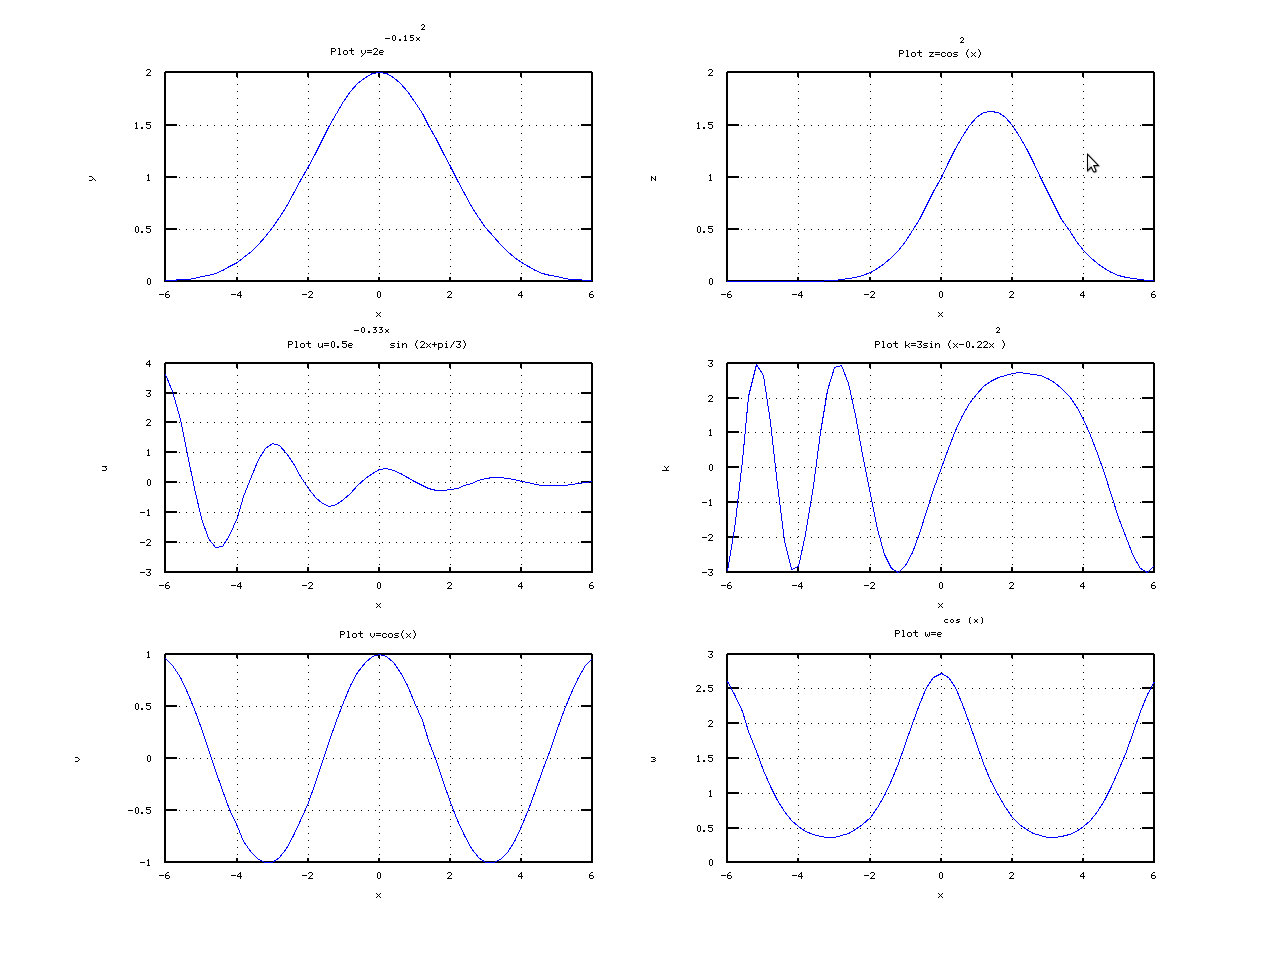
\includegraphics[width=8cm]{04_aer_octave_fig1.png}}
\caption{Графики графики нескольких функций в одном окне}
\label{pic:1}
\end{figure}

\begin{figure}[ht]
\centering{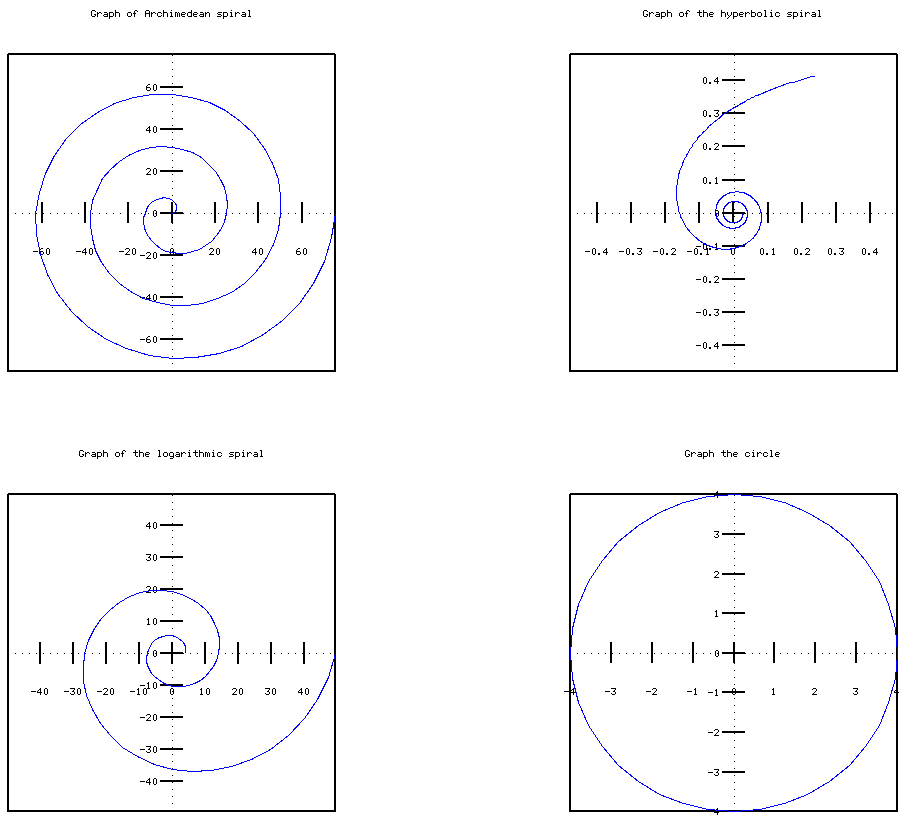
\includegraphics[width=8cm]{04_aer_octave_fig2.png}}
\caption{ Графики архимедовой, гиперболической и логарифмической спирали, окружности в полярных координатах}
\label{pic:2}
\end{figure}

\begin{figure}[ht]
\centering{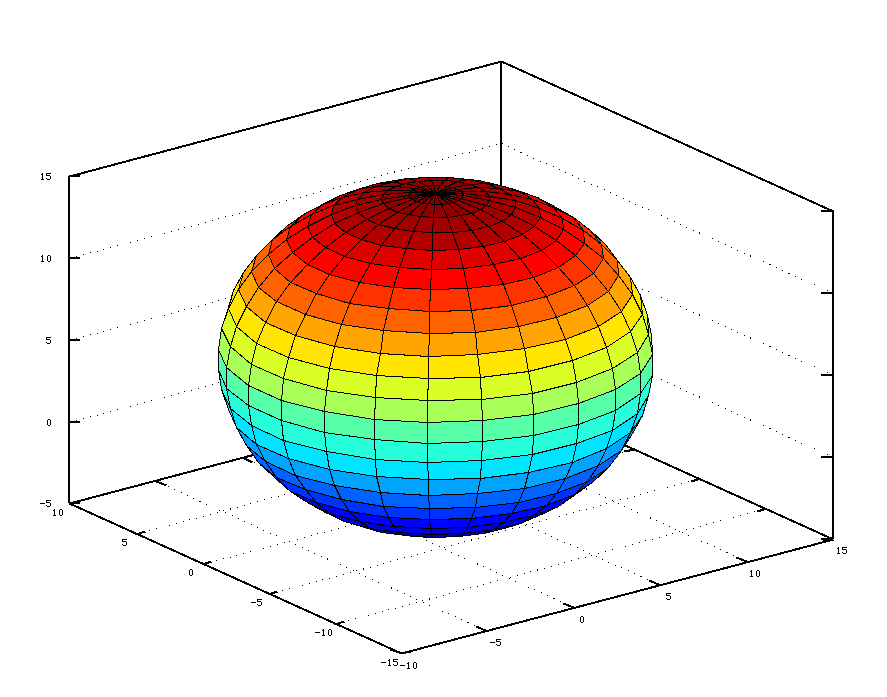
\includegraphics[width=8cm]{04_aer_octave_fig3.png}}
\caption{График сферы}
\label{pic:3}
\end{figure}

Octave содержит большое количество функций, предназначенных для решения задач линейной алгебры, наиболее используемые из них: \verb!det(M)! --- вычисляет определитель квадратной матрицы \verb!M!, \verb!norm(M[,p])! --- возвращает различные виды норм матрицы \verb!M! в зависимости от \verb!p!, \verb!inv(M)! --- возвращает матрицу обратную к \verb!M!, \verb!eig(M)! --- возвращает вектор собственных значений матрицы \verb!M!, \verb!rref(M)! --- осуществляет приведение матрицы \verb!M! к треугольной форме, используя метод исключения Гаусса, \verb!lu(M)!, \verb!qr (M)! --- выполняют LU и QR-разложение соответственно. 

Мощная графическая и математическая база  Octave позволяет решать задачи векторной алгебры и аналитической геометрии.

Octave содержит функции для численного и аналитического решения нелинейных уравнений и систем, а также для интегрирования и дифференцирования.

Оптимизационные задачи чаще всего решают с помощью проприетарного табличного процессора MS Excel. Однако, наиболее мощные и гибкие функции для решения подобных задач присутствуют именно в Octave. Так, для  решения линейных и нелинейных оптимизационных задач с ограничениями можно использовать функцию sqp, а для решения любых задач линейного программирования есть функция glpk. Сложные оптимизационные задачи в Octave решают с помощью пакета пакета расширений Minimization для GNU Octave (\url{http://octave.sourceforge.net/optim/overview.html}).

В инженерной практике часто приходится сталкиваться с решением обыкновенных дифференциальных уравнений и систем. В Octave существует достаточно много функций для решения обыкновенных уравнений и систем (в том числе и жёстких). Наиболее часто используемые среди них:
\begin{itemize}
\item \verb!ode23!, \verb!ode45! --- функции решений обыкновенных нежёстких дифференциальных уравнений (или систем) методом Рунге-Кутта 2-3-го и 4-5-го порядка точности соответсвенно,
\item \verb!ode5r!, \verb!ode2r! --- функции решений обыкновенных жёстких дифференциальных уравнений (или систем).
\end{itemize}

\begin{figure}[ht]
\centering{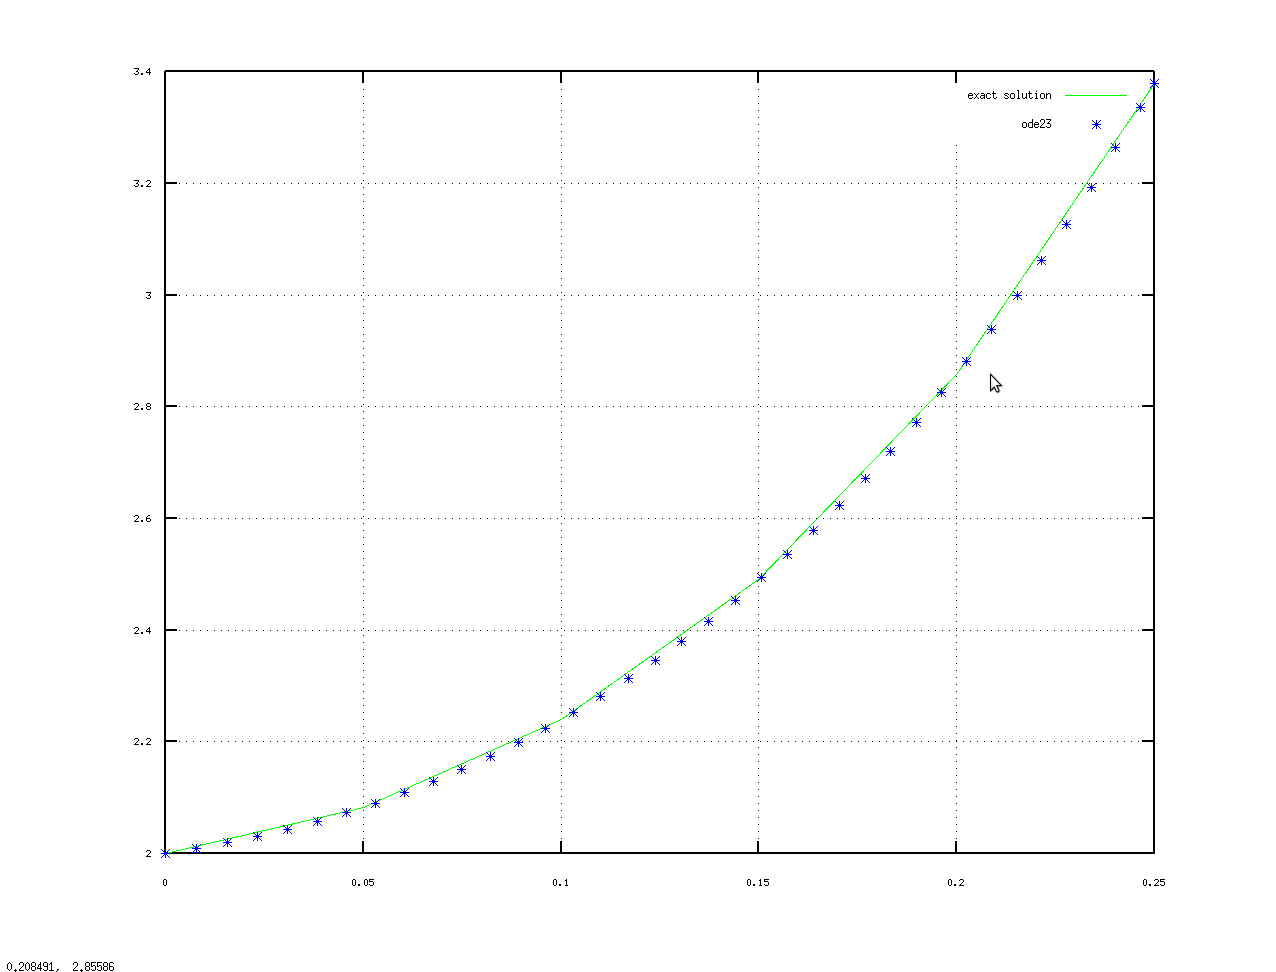
\includegraphics[width=8cm]{04_aer_octave_fig4.png}}
\caption{Графики точного решения (--) дифференциального уравнений и решения (*), найденного с помощью ode23}
\label{pic:4}
\end{figure}

Множество функций для решения дифференциальных уравнений находится в пакете расширений odepkg. Краткое описание функций этого пакета на английском языке с некоторыми примерами приведено на странице \url{http://octave.sourceforge.net/odepkg/overview.html}.

Также в Octave можно решать практически любые задачи обработки эксперимента. Для подбора параметров аналитической зависимости методом наименьших квадратов используются следующие функции: \verb!polyfit! --- подбор коэффициентов полинома k-й степени; \verb!sqp! --- функция поиска минимума.

Сплайн-интерполяция в Octave реализуется с помощью функции \verb!interp1!, которая позволяет  построить кубический и линейный сплайн.

C помощью Octave можно решать и много других задач. Авторами подготовлен учебник по использованию пакете GNU Octave, который будет опубликован в ближайшее время в Москве, в серии учебников ALT Linux, а также небольшим тиражом в Донецком национальном техническом университете. Рабочие материалы книги можно увидеть на сайте \url{http://gnu-octave.narod2.ru}.

Рассмотренные возможности Octave позволяют авторам рекомендовать пакет как инструмент для решения математических задач в курсах <<Высшая математика>>, <<Математический анализ>>, <<Линейная алгебра>>, <<Аналитическая геометрия>>, а также во многих специальных курсах, в которых приходится решать задачи вычислительной математики.
\end{document}





\documentclass[10pt, a5paper]{article}
\usepackage{pdfpages}
\usepackage{parallel}
\usepackage[T2A]{fontenc}
\usepackage{ucs}
\usepackage[utf8x]{inputenc}
\usepackage[polish,english,russian]{babel}
\usepackage{hyperref}
\usepackage{rotating}
\usepackage[inner=2cm,top=1.8cm,outer=2cm,bottom=2.3cm,nohead]{geometry}
\usepackage{listings}
\usepackage{graphicx}
\usepackage{wrapfig}
\usepackage{longtable}
\usepackage{indentfirst}
\usepackage{array}
\newcolumntype{P}[1]{>{\raggedright\arraybackslash}p{#1}}
\frenchspacing
\usepackage{fixltx2e} %text sub- and superscripts
\usepackage{icomma} % коскі ў матэматычным рэжыме
\PreloadUnicodePage{4}

\newcommand{\longpage}{\enlargethispage{\baselineskip}}
\newcommand{\shortpage}{\enlargethispage{-\baselineskip}}

\def\switchlang#1{\expandafter\csname switchlang#1\endcsname}
\def\switchlangbe{
\let\saverefname=\refname%
\def\refname{Літаратура}%
\def\figurename{Іл.}%
}
\def\switchlangen{
\let\saverefname=\refname%
\def\refname{References}%
\def\figurename{Fig.}%
}
\def\switchlangru{
\let\saverefname=\refname%
\let\savefigurename=\figurename%
\def\refname{Литература}%
\def\figurename{Рис.}%
}

\hyphenation{admi-ni-stra-tive}
\hyphenation{ex-pe-ri-ence}
\hyphenation{fle-xi-bi-li-ty}
\hyphenation{Py-thon}
\hyphenation{ma-the-ma-ti-cal}
\hyphenation{re-ported}
\hyphenation{imp-le-menta-tions}
\hyphenation{pro-vides}
\hyphenation{en-gi-neering}
\hyphenation{com-pa-ti-bi-li-ty}
\hyphenation{im-pos-sible}
\hyphenation{desk-top}
\hyphenation{elec-tro-nic}
\hyphenation{com-pa-ny}
\hyphenation{de-ve-lop-ment}
\hyphenation{de-ve-loping}
\hyphenation{de-ve-lop}
\hyphenation{da-ta-ba-se}
\hyphenation{plat-forms}
\hyphenation{or-ga-ni-za-tion}
\hyphenation{pro-gramming}
\hyphenation{in-stru-ments}
\hyphenation{Li-nux}
\hyphenation{sour-ce}
\hyphenation{en-vi-ron-ment}
\hyphenation{Te-le-pathy}
\hyphenation{Li-nux-ov-ka}
\hyphenation{Open-BSD}
\hyphenation{Free-BSD}
\hyphenation{men-ti-on-ed}
\hyphenation{app-li-ca-tion}

\def\progref!#1!{\texttt{#1}}
\renewcommand{\arraystretch}{2} %Іначай формулы ў матрыцы зліпаюцца з лініямі
\usepackage{array}

\def\interview #1 (#2), #3, #4, #5\par{

\section[#1, #3, #4]{#1 -- #3, #4}
\def\qname{LVEE}
\def\aname{#1}
\def\q ##1\par{{\noindent \bf \qname: ##1 }\par}
\def\a{{\noindent \bf \aname: } \def\qname{L}\def\aname{#2}}
}

\def\interview* #1 (#2), #3, #4, #5\par{

\section*{#1\\{\small\rm #3, #4. #5}}

\def\qname{LVEE}
\def\aname{#1}
\def\q ##1\par{{\noindent \bf \qname: ##1 }\par}
\def\a{{\noindent \bf \aname: } \def\qname{L}\def\aname{#2}}
}


\begin{document}
\renewcommand{\figurename}{Рыс.} % Не перакідаць у прэамбулу --- не працуе, чаму -- халера ведае.
\renewcommand{\abstractname}{Анатацыя}
\renewcommand{\refname}{Літаратура}

\title{Выкарыстанне свабоднага праграмнага забеспячэння ва ўстановах адукацыі Украіны: спроба аналізу}

\author{Грыгорый Злобiн\footnote{Львоўскі нацыянальны ўніверсітэт ім. Івана Франка, \url{zlobin@electronics.wups.lviv.ua}}}
\date{}

\maketitle

\begin{abstract}
The analysis of free / open source software usage in higher educational institutions of Ukraine is presented, based of the `FOSS Lviv-2011'  International Scientific Conference reports. 
\end{abstract}

Нягледзячы на станоўчы досвед выкарыстання свабодных праграм у адукацыі як у краінах блізкага, так і далёкага замежжа, ва Украіне да гэтага часу не прынятая канцэпцыя выкарыстання свабоднага праграмнага забеспячэння у адукацыі. Разам з тым намаганнямі энтузіястаў у навучальных установах Украіны свабоднае праграмнае забеспячэнне ўсё ж выкарыстоўваецца! Праз адасобленую пазіцыю Міністэрства адукацыі і навукі Украіны няма падрабязнай інфармацыі аб досведзе выкарыстання свабодных праграм у адукацыі. Дзякуючы таму, што ў Львоўскім нацыянальным універсітэце імя Івана Франка 01--06 лютага 2011 адбылася даволі прадстаўнічая міжнародная навукова"=практычная канферэнцыя <<FOSS Lviv-2011>>, з'явілася магчымасць правядзення аналізу выкарыстання СПЗ у вышэйшых навучальных установах Украіны. З 81 дакладаў 49 было прысвечана выкарыстанню СПЗ у навучальных установах. Даклады \cite{fosslviv}, якія былі пададзеныя на гэтую канферэнцыю, можна згрупаваць па наступных кірунках (назва дакладу падаецца на мове арыгіналу):

\section*{Дыстанцыйнае навучанне}
Гэтай тэматыцы прысвечаная найбольшая колькасць дакладаў "--- 10:
\begin{itemize}
\item <<Розроблення електронного деканату для системи управління дистанційним навчання MOODLE>> --- Артеменко В.Б., Львоўская камерцыйная акадэмія
\item <<Вибір платформи дистанційного навчання>> --- Коцаренко М.В., Бойко О.В.,  Львоўскі нацыянальны медыцынскі ўніверсітэт ім. Данііла Галіцкага
\item <<Використання контрольно-діагностичної програми iTest у ході моніторингу якості процесу навчання старшокласників>> --- Макаренко І.Є., Мерзлікін П.В., Крыварожскі дзяржаўны педагагічны ўніверсітэт
\item  <<Використання системи Moodle для організації контролю знань майбутніми вчителями-гуманітаріями>> --- Маркова Є.С., Бердзянскі дзяржаўны педагагічны ўніверсітэт
\item  <<Тестування в  Moodle як елемент менеджменту якості освіти: перший досвід>> --- Сергієнко В.П., Сліпухіна І.А., НПУ ім. М.П. Драгаманава
\item  <<Особливості програмного забезпечення в електронному навчанні>> --- Жарких Ю.С., Лисоченко С.В., Сусь Б.Б., Третяк О.В., Кіеўскі нацыянальны ўніверсітэт ім. Тараса Шаўчэнкі
\item  <<Інформаційно-аналітична система управління навчальним процесом ВНЗ на базі  Moodle>> --- Триус Ю.В., Чаркаскі дзяржаўны тэхналагічны ўніверсітэт
\item  <<Використання CMS JOMLA!  та LCMS MOODLE у ВНЗ>> --- Франчук В.М., НПУ ім. М.П. Драгаманава
\item <<Локалізація системи MOODLE " --- Франчук В.М., НПУ ім. М.П. Драгаманава
\item  <<Застосування вільного програмного забезпечення для дистанційного навчання у вищих навчальних закладах>> --- Захарченко В.М., Шапо В.М., Адэская нацыянальная марская акадэмія
\end{itemize}
\newpage

\section*{Выкарыстанне сістэм кампутарнай матэматыкі}
Наступныя 6 дакладаў можна аднесці да матэматычнай тэматыкі:
\begin{itemize}
\item <<Використання вільно-поширюваного ПЗ математичного призначення в університеті>> "--- Бугаєць Н.О., НПУ ім. М.П. Драгаманава
\item <<Вільнопоширювані системи комп'ютерної математики в осві\-ті і науці>> "--- Лазурчак І.І., Кобильник Т.П., Драгобыцкі дзяржаўны ўніверсітэт ім. І. Франка
\item <<Використання комп'ютерних математичних систем у про\-фе\-сій\-ній підготовці майбутнього вчителя математики>> "--- Лов'я\-но\-ва І.В., Крыварожскі дзяржаўны педагагічны ўніверсітэт
\item <<Моделювання задач електротехніки у XCOS>> "--- Філь І.М., Данецкі нацыянальны тэхнічны ўніверсітэт
\item <<Розробка і використання web-інтерфейсів для роботи з системами комп'ютерної математики>> "--- Чичкарьов Є.А., Прыазоўскі дзяржаўны тэхнічны ўніверсітэт
\item <<Про комп'ютерний супровід викладання геометрії>> "--- Яхненко І.В., Лутфулін М.В., Палтаўскі нацыянальны педагагічны ўніверсітэт ім. В.Г. Караленкі
\end{itemize}

\section*{Агульныя пытанні выкарыстання СПЗ у адукацыі}
7 дакладаў гэтай групы, якую можна прызнаць другой па колькасці, уключалі:
\begin{itemize}
\item <<Використання вільного програмного забезпечення в навчанні і наукових дослідженнях у Львівському національному уні\-вер\-ситеті імені Івана Франка>> "--- Апуневич С.Є., Злобін Г.Г., Рикалюк Р.Є., Шувар Р.Я., Львоўскі нацыянальны ўніверсітэт ім. І. Франка
\item <<Використання вільного програмного забезпечення в системі дистанційної освіти>> "--- Воронкін О.С., Луганскі дзяржаўны інстытут культуры і мастацтваў
\item <<Вільнопоширюване програмне забезпечення курсу “Нові інформаційні технології” для студентів спеціальності \linebreak “Біо\-ло\-гія”>> "--- Єфименко В.В., НПУ ім. М.П. Драгаманава
\item <<Використання вільного програмного забез\-печення у про\-фе\-сій\-ній підготовці майбутніх інженерів>> "--- Покришень Д.А., \linebreak Дрозд О.П., Сподаренко І.Й., Чарнігаўскі дзяржаўны тэхналагічны ўніверсітэт
\item  <<Про досвід використання ОС Linux у навчальному процесі Львівського національного медичного університету імені Данила Галицького>> "--- Риковський П.А., Львоўскі нацыянальны медыцынскі ўніверсітэт ім. Данііла Галіцкага
\item  <<LINUX  та VIRTUAL-BOX у навчанні абстрактних понять теорії операційних систем>> "--- Спірін О.М., Сверчевська О.С., Жытомірскі дзяржаўны ўніверсітэт ім. І. Франка
\item  <<З досвіду використання вільного програмного забезпечення при вивченні інформатики>> "--- Харченко В.М., Нежынскі дзяржаўны ўніверсітэт ім. М. Гогаля
\end{itemize}

\section*{Выкарыстанне адкрытых сродкаў праграмавання}
Гэтая група апынулася найменшай па колькасці і ўключае 4 даклады:
\begin{itemize}
\item <<Використання відкритих програмних засобів в процесі навчання статистичним дисциплінам>> "--- Коркуна Т.Й., Самбарскі тэхнікум эканомікі і інфарматыкі
\item <<Розрахунок фотоіонізаційних моделей небулярного газу в ОС LINUX UBUNTU 10.10 та WINDOWS 7>> "--- Мелех Б.Я., Тишко Н.Л., Коритко Р.І., Львоўскі нацыянальны ўніверсітэт ім. І. Франка
\item <<Реалізація розподілених обчислень на основі грід-платформи з відкритим кодом BOINC>> "--- Шийка Ю.Я., Шувар Р.Я., \linebreak Львоўскі нацыянальны ўніверсітэт ім. І. Франка
\item <<Реалізація високопродуктивної обчислювальної системи на базі ОС  LINUX>> "--- Шувар Р.Я., Бойко Я.В., Львоўскі нацыянальны ўніверсітэт ім. І. Франка
\end{itemize}

\section*{Распрацоўка праграмнага забеспячэння}
Будучы тэматычна-роднаснай папярэдняй, гэтая група больш шматлікая і складаецца з 7 дакладаў, яна зраўнавалася з катэгорыяй <<Агульныя пытанні выкарыстання СПЗ у адукацыі>>:
\begin{itemize}
\item <<Комплекс програм для лазерних спостережень штучних супутників Землі>> "--- Мартинюк-Лотоцький К.П., Білінський\linebreak А.\,І., Львоўскі нацыянальны ўніверсітэт ім. І. Франка
\item <<Розробка системи спектральної діагностики димової плазми>> "--- Сподарець Д.В., Драган Г.С., Адэскі нацыянальны ўні\-версітэт імя І.І. Мечнікава
\item <<Використання вільного програмного забез-печення для створення програми керування інформаційним автоматом>> "--- Зло\-бін Г., Скляр В., Чмихало О., Шевчик В., Львоўскі нацыянальны ўніверсітэт ім. І. Франка
\item <<Використання бібліотеки класів GEANT4 в ОС Linux при розробці програмного забезпечення для моделювання процесів взаємодії випромінювання з речовиною>> "--- Малихіна Т.В., Харкаўскі нацыянальны ўніверсітэт ім. В.Н. Каразіна
\item  <<Програма для обробкирезультатів ЛЛС-спостережень як \linebreak ВПЗ>> "--- Апуневич С.Є., Апуневич С.В., Білінський А.І., Благодир Я.Т., Львоўскі нацыянальны ўніверсітэт ім. І. Франка
\item  <<Програмне забезпечення керування телескопом  ЛЛС-станції Львів-1831>> "--- Білінський А.І., Мартинюк-Лотоцький К.\,П., \linebreak Львоўскі нацыянальны ўніверсітэт ім. І. Франка
\item <<Використання Open Wrt як основи вбудованого програмного забезпечення маршрутизаторів>> "--- Нек Т., Львоўскі нацыянальны ўніверсітэт ім. І. Франка
\end{itemize}

\section*{Асобныя даклады}
І нарэшце, 5 дакладаў немагчыма аднесці ні да адной з пералічаных вышэй катэгорый:
\begin{itemize}
\item  <<Інформаційна технологія управління навчальним навантаженням у вищих навчальних закладах>> "--- Гриценко В.Г., Чаркаскі нацыянальны ўніверсітэт ім. Б. Хмяльніцкага
\item  <<Про досвід використання офісного  пакету OpenOffice.org.ukr в курсі інформатики для економічних і юридичних спеціальностей ВЗО>> "--- Злобін Г.Г., Львоўскі нацыянальны ўніверсітэт ім. І. Франка 
\item  <<Досвід використання  редактора Gimp при вивченні курсу “Комп'ютерна графіка і дизайн”>> "--- Матвієнко Ю.С., Палтаўскі нацыянальны педагагічны ўніверсітэт ім. В.Г. Караленкі
\item <<Використання програми GANTTPROJECT для побудови календарних графіків при розробці ПВР>> "--- Грицук Ю.В., Меліхов О.І., Данбаская акадэмія будаўніцтва і архітэктуры
\item <<Вільне ПЗ для підготовки наукових текстів і презентацій>> "--- Лутфуллін М.В., Моторний М.І., Палтаўскі нацыянальны педагагічны ўніверсітэт ім. В.Г. Караленкі
\end{itemize}

	Такім чынам, можна канстатаваць як шырокі спектр выкарыстання СПЗ ва ўкраінскіх навучальных установах ад дыстанцыйнага навучання да распрацоўкі адкрытага праграмнага забеспячэння, так і шырокую геаграфію выкарыстання СПЗ ад Луганска на ўсходзе да Львова на захадзе і ад Чарнігава на поўначы да Адэсы на поўдні (глядзі рыс.).

\begin{figure}[ht]
\centering{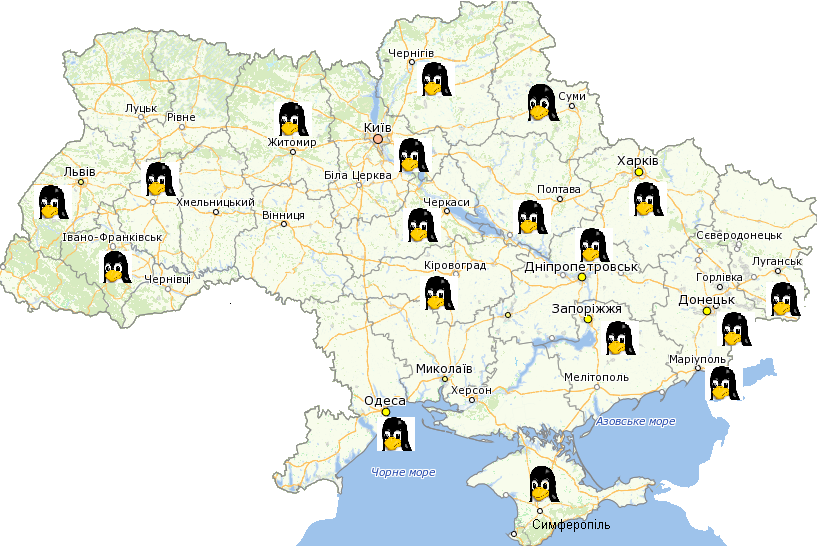
\includegraphics[width=8cm]{05_ukraine_linux.png}}
\label{pic:fl1}
%\caption{~}
\end{figure}

\begin{thebibliography}{9}
\bibitem{fosslviv}Тези міжнародної науково-практичної конференції FOSS LVIV-2011. Збірник наукових праць /за ред. Злобіна Г.Г., Апуневича С.Є., Машкова В.В., Апуневич С.В. Вид-во ЛНУ імені Івана Франка. 2011. --- 196 с.
\end{thebibliography}

\end{document}





\documentclass[a5paper,10pt]{article}
\usepackage{pdfpages}
\usepackage{parallel}
\usepackage[T2A]{fontenc}
\usepackage{ucs}
\usepackage[utf8x]{inputenc}
\usepackage[polish,english,russian]{babel}
\usepackage{hyperref}
\usepackage{rotating}
\usepackage[inner=2cm,top=1.8cm,outer=2cm,bottom=2.3cm,nohead]{geometry}
\usepackage{listings}
\usepackage{graphicx}
\usepackage{wrapfig}
\usepackage{longtable}
\usepackage{indentfirst}
\usepackage{array}
\newcolumntype{P}[1]{>{\raggedright\arraybackslash}p{#1}}
\frenchspacing
\usepackage{fixltx2e} %text sub- and superscripts
\usepackage{icomma} % коскі ў матэматычным рэжыме
\PreloadUnicodePage{4}

\newcommand{\longpage}{\enlargethispage{\baselineskip}}
\newcommand{\shortpage}{\enlargethispage{-\baselineskip}}

\def\switchlang#1{\expandafter\csname switchlang#1\endcsname}
\def\switchlangbe{
\let\saverefname=\refname%
\def\refname{Літаратура}%
\def\figurename{Іл.}%
}
\def\switchlangen{
\let\saverefname=\refname%
\def\refname{References}%
\def\figurename{Fig.}%
}
\def\switchlangru{
\let\saverefname=\refname%
\let\savefigurename=\figurename%
\def\refname{Литература}%
\def\figurename{Рис.}%
}

\hyphenation{admi-ni-stra-tive}
\hyphenation{ex-pe-ri-ence}
\hyphenation{fle-xi-bi-li-ty}
\hyphenation{Py-thon}
\hyphenation{ma-the-ma-ti-cal}
\hyphenation{re-ported}
\hyphenation{imp-le-menta-tions}
\hyphenation{pro-vides}
\hyphenation{en-gi-neering}
\hyphenation{com-pa-ti-bi-li-ty}
\hyphenation{im-pos-sible}
\hyphenation{desk-top}
\hyphenation{elec-tro-nic}
\hyphenation{com-pa-ny}
\hyphenation{de-ve-lop-ment}
\hyphenation{de-ve-loping}
\hyphenation{de-ve-lop}
\hyphenation{da-ta-ba-se}
\hyphenation{plat-forms}
\hyphenation{or-ga-ni-za-tion}
\hyphenation{pro-gramming}
\hyphenation{in-stru-ments}
\hyphenation{Li-nux}
\hyphenation{sour-ce}
\hyphenation{en-vi-ron-ment}
\hyphenation{Te-le-pathy}
\hyphenation{Li-nux-ov-ka}
\hyphenation{Open-BSD}
\hyphenation{Free-BSD}
\hyphenation{men-ti-on-ed}
\hyphenation{app-li-ca-tion}

\def\progref!#1!{\texttt{#1}}
\renewcommand{\arraystretch}{2} %Іначай формулы ў матрыцы зліпаюцца з лініямі
\usepackage{array}

\def\interview #1 (#2), #3, #4, #5\par{

\section[#1, #3, #4]{#1 -- #3, #4}
\def\qname{LVEE}
\def\aname{#1}
\def\q ##1\par{{\noindent \bf \qname: ##1 }\par}
\def\a{{\noindent \bf \aname: } \def\qname{L}\def\aname{#2}}
}

\def\interview* #1 (#2), #3, #4, #5\par{

\section*{#1\\{\small\rm #3, #4. #5}}

\def\qname{LVEE}
\def\aname{#1}
\def\q ##1\par{{\noindent \bf \qname: ##1 }\par}
\def\a{{\noindent \bf \aname: } \def\qname{L}\def\aname{#2}}
}


\begin{document}


\title{Облачные вычисления и сервисы: классификация, основные функции, преимущества и недостатки}

\author{Виталий Сороко\footnote{Минск, \url{http://arneta.ru}}}

\maketitle
\begin{abstract}
In the past, big part of computer-related activity was impos\-sible without the installation of software to a local computer, but now, with help of cloud services, users can perform such typical tasks as word processing within their web-browser. It becomes possible due to so called cloud-based resources. Here an attempt of  cloud technologies and systems general overview is presented with the technical description of the architecture, characteristics and features comparison. 
\end{abstract}

Среди наиболее полных определений облачных систем на сегодняшний день можно выделить следующие два:
\begin{itemize}
\item Облачные сервисы "--- это технология обработки данных, в которой программное обеспечение предоставляется пользователю как интернет-сервис, при котором от пользователя скрыта инфраструктура <<облака>> (облачной системы) и, поэтому, ему не требуются специальные знания и навыки для  управления и использования данной <<облачной>> технологии.
\item Облачные вычисления "--- это вычисления, которые представляют собой динамически масштабируемый способ доступа к внешним вычислительным ресурсам в виде сервиса, предоставляемого посредством Интернета.
\end{itemize}

Данные определения тесно связаны между собой: для реализации всех облачных сервисов необходимы вычисления, а облачные вычисления по сути сами являются облачным сервисом. Рассмотрим классификацию облачных сервисов и их реализаций из мира свободного ПО.

В настоящее время все облачные сервисы подразделяют на:
\begin{itemize}
\item \emph{«Программное обеспечение как услуга»} (Software as a Service, сокращённо SaaS) "--- бизнес-модель продажи программного \linebreak обеспечения, при которой владелец (поставщик) ПО предоставляет доступ к к нему пользователям (заказчикам) через Интернет. Примерами такого ПО являются Feng Office Community Edition, Simple Groupware, Zarafa и др.
\item \emph{«Оборудование (вычислительные мощности) как услуга»} \linebreak (Hardware as a Service, сокращённо HaaS) "--- предоставление  вычислительных ресурсов оборудования (его процессорного времени, места для место под хранения данных и т.д.) в виде сервисов с использованием технологий виртуализации. Сервисы обычно предлагаются как эквивалент реальным вычислительным системам, таким как серверы, суперкомпьютеры и др. Над программной реализацией этой идеи полностью или частично работают проекты OpenVZ, FreeVPS, Linux-VServer, Apache Hama, GlusterFS Open Source Project, а также Moose File System (MooseFS) и др., а предоставляет такой сервис на базе OpenSource решений компания Linode и некоторые другие.
\item \emph{<<Коммуникация как Сервис>>} (Communications as a Service, сокр. CaaS) "--- построенное в облаке коммуникационное решение для предприятия, которое обеспечивает передачу речевого сигнала по сети Интернет или по любым другим IP-сетям (VoIP), обмен мгновенными сообщениями (IM), видеоконференции. Модель CaaS позволяет деловым клиентам выборочно разворачивать средства коммуникаций и услуг на оснований оплаты услуг в срок для используемых сервисов. С этим направлением тесно связаны такие FOSS-проекты как Ekiga, iLBC, Speex.
\item \emph{«Мониторинг как Сервис»} (Monitoring-as-a-Service, сокращённо MaaS) является обслуживаемым в облаке программным обеспечением для мониторинга и обеспечения безопасности. Такими OpenSource-решениями на сегодняшний день являются Ganglia, Zabbix, Hyperic HQ. Сюда же  с некоторыми оговорками модно отнести и Nagios. 
\item \emph{«Инфраструктура как услуга»} (Infrastructure as a Service, сокращённо IaaS) "--- это предоставление компьютерной инфраструктуры (как правило в форме виртуализации) как услуги на основе концепции облачных вычислений. По сути IaaS является комбинацией SaaS,  HaaS, так как она включает в себя и то и другое, причем обычно во множественном числе, а также CaaS и иногда MaaS с целью объедения и мониторинга всей системы, и, поэтому, используется в основном предприятиями. Свободными реализациями данной концепции являются Eucalyptus, OpenNebula, OpenStack, Nimbus и др.
\item \emph{«Платформа как услуга»} (Platform as a Service, сокр. PaaS) "--- предоставление программной платформы и инструментов с определенными характеристиками, необходимых для разработки, тестирования, развертывания, поддержки различных приложений. Сюда же входят и готовые к использованию облачные сервисы, которые вместе образуют программную платформу. Яркими примерами из мира OpenSource в настоящее время являются Xen Cloud Platform, Cloud Foundry, Apache Hadoop, Apache Hive и др.
\item \emph{«Компьютер (виртуальный рабочий стол) как услуга»} (Desk\-top as a Service, сокращённо DaaS) "--- предоставление виртуального компьютера, который каждый пользователь может индивидуально настраивать под свои задачи. Таким образом, пользователь приходя на работу просто вводит свои данные (обычно логин и пароль) и может работать, используя при этом благодаря технологиям виртуализации вычислительные мощности стороннего сервера, а не своего ПК. 
\item \emph{<<Рабочее окружение как услуга>>} (Workspace as a Service, сокращённо WaaS) "--- предоставление комплекта  SaaS, предназначенного для создания рабочего окружения. В отличие от DaaS в этом случае пользователь получает доступ только к ПО, в то время как все вычисления происходят непосредственно на его машине. По сути данная категория является гибридом SaaS и PaaS, так как в отличие от последней является платформой, направленной не на разработку и тестирование ПО, а на офисную работу, но при этом как первая в реализации не использует технологий виртуализации. На данный момент реализации данной технологии предоставляются в основном различными крупными компаниями, например Google и Microsoft, и представляют в основном решения с закрытым исходным кодом, иногда с использованием свободных и открытых компонентов или их исходников.
\item \emph{«Все как услуга»} (Everything as a service, сокращённо EaaS) "--- концептуальная модель, включающая в себя элементы всех перечисленных решений. На данный момент полной её реализации не существует "--- она по сути является идеалом для крупных облачных компаний, таких как Google и Microsoft.
\end{itemize}

Свободное и открытое программное обеспечение в настоящее время играет ключевую роль в создании и развертывании облачных сервисов и систем. С одной стороны существуют ряд созданных сообществом платформ, ориентированных на облачные вычисления (Xen, Eucaliptus, Cloud Foundry, Feng Office и др.). С другой стороны, само свободное ПО (операционные системы семейства Linux и BSD, Web-браузеры и т.\,д.) как нельзя лучше подходит для размещения и использования облачных сервисов.  Естественно, что существует и целый ряд проприетарных аналогов.

Рыночная доля облачных сервисов и платформ постоянно растет благодаря ряду преимуществ для обычных пользователей и организаций, среди которых в первую очередь можно отметить:
\begin{itemize}
\item	количество процессоров, объем оперативной памяти и дискового пространства в облачных системах теоретически ничем не ограничен;
\item	пользователям не нужно самостоятельно устанавливать и настраивать ПО, т.\,к. для доступа к облачным сервисам достаточно обычного web-браузера;
\item	пользователям не нужно покупать дорогое оборудование;
\item	экономия времени и энергии на выполнение некоторых задач, а также, в особых случаях, и площадей, занимаемых оборудованием;
\item	возможность производить оплату только за потребленные вычислительные мощности и произведенные операции;
\item	в организациях отсутствуют затраты на развёртывание инфраструктуры;
\item	организации получают сокращение затрат на техническую поддержку и обновление развернутых систем, а также высокую скорость внедрения, обусловленную отсутствием временных затрат на развертывание системы;
\item	отсутствует необходимость обучения "--- большинство пользователей уже умеют пользоваться web-браузерами и интернет-сервисами как классом услуг;
\item	обычно облачные системы обслуживаются высококвалифицированными профессионалами, что дает более высокий уровень качества обслуживания ПО.
\end{itemize}

Тем не менее облачные системы не лишены недостатков, которые в большей степени касаются обычных пользователей, и в меньшей --- провайдеров:
\begin{itemize}
\item из-за вопросов безопасности не все данные можно доверить стороннему провайдеру, тем более, не только для хранения, но и для обработки;
\item далеко не каждое облачное приложение позволяет сохранить полученные результаты в удобном для пользователя виде на нужный носитель данных;
\item риск массовой потери данных многими пользователями из-за технического сбоя у поставщика облачных услуг;
\item потеря свободы "--- большая часть облачных сервисов не имеет четких стандартов, и поэтому при переходе от одного поставщика облачных услуг к другому могут возникнуть серьезные проблемы. Они же могут возникнуть и при обновлении провайдером собственных облачных сервисов "--- если, например, он пожелает внедрить новый интерфейс, то подписчикам придётся им пользоваться.  Немаловажным моментом также является необходимость доступа в интернет, что в некоторых случаях ведет к потере свободы перемещений. А главное, благодаря тому, что все данные находятся в руках провайдера, нельзя исключать того, что недобросовестные компании могут воспользоваться этим.
\end{itemize}

Можно предположить, что как сейчас большая часть пользователей использует Windows и Microsoft Office, так в ближайшем будущем эти пользователи оценят преимущества облачных платформ и перейдут на них. При этом, даже передумав после получения очередной порции счетов за оплату сервисов, пользователям будет трудно вернуться к прежней схеме работы "--- все их данные будут в руках компании"=владельца облачной системы, а для самостоятельной установки другой операционной системы и иного программного обеспечения многим не хватит квалификации, да и приобретённое пользователями оборудование скорее всего будет иметь крайне малую мощность. В этом случае эффективным выходом оказывается  свободное ПО, которое как правило способно работать на маломощном оборудовании при сохранении совместимости со старыми системами. В этом случае возврат пользователей из облака также едва ли станет массовым, поскольку крупные облачные компании постараются сделать этот переход невыгодным, если не невозможным, однако сам факт такой возможности будет являться дополнительным регулирующим фактором, ограничивающим прибыли провайдеров облачных услуг.

\end{document}

\documentclass[10pt, a5paper]{article}
\usepackage{pdfpages}
\usepackage{parallel}
\usepackage[T2A]{fontenc}
\usepackage{ucs}
\usepackage[utf8x]{inputenc}
\usepackage[polish,english,russian]{babel}
\usepackage{hyperref}
\usepackage{rotating}
\usepackage[inner=2cm,top=1.8cm,outer=2cm,bottom=2.3cm,nohead]{geometry}
\usepackage{listings}
\usepackage{graphicx}
\usepackage{wrapfig}
\usepackage{longtable}
\usepackage{indentfirst}
\usepackage{array}
\newcolumntype{P}[1]{>{\raggedright\arraybackslash}p{#1}}
\frenchspacing
\usepackage{fixltx2e} %text sub- and superscripts
\usepackage{icomma} % коскі ў матэматычным рэжыме
\PreloadUnicodePage{4}

\newcommand{\longpage}{\enlargethispage{\baselineskip}}
\newcommand{\shortpage}{\enlargethispage{-\baselineskip}}

\def\switchlang#1{\expandafter\csname switchlang#1\endcsname}
\def\switchlangbe{
\let\saverefname=\refname%
\def\refname{Літаратура}%
\def\figurename{Іл.}%
}
\def\switchlangen{
\let\saverefname=\refname%
\def\refname{References}%
\def\figurename{Fig.}%
}
\def\switchlangru{
\let\saverefname=\refname%
\let\savefigurename=\figurename%
\def\refname{Литература}%
\def\figurename{Рис.}%
}

\hyphenation{admi-ni-stra-tive}
\hyphenation{ex-pe-ri-ence}
\hyphenation{fle-xi-bi-li-ty}
\hyphenation{Py-thon}
\hyphenation{ma-the-ma-ti-cal}
\hyphenation{re-ported}
\hyphenation{imp-le-menta-tions}
\hyphenation{pro-vides}
\hyphenation{en-gi-neering}
\hyphenation{com-pa-ti-bi-li-ty}
\hyphenation{im-pos-sible}
\hyphenation{desk-top}
\hyphenation{elec-tro-nic}
\hyphenation{com-pa-ny}
\hyphenation{de-ve-lop-ment}
\hyphenation{de-ve-loping}
\hyphenation{de-ve-lop}
\hyphenation{da-ta-ba-se}
\hyphenation{plat-forms}
\hyphenation{or-ga-ni-za-tion}
\hyphenation{pro-gramming}
\hyphenation{in-stru-ments}
\hyphenation{Li-nux}
\hyphenation{sour-ce}
\hyphenation{en-vi-ron-ment}
\hyphenation{Te-le-pathy}
\hyphenation{Li-nux-ov-ka}
\hyphenation{Open-BSD}
\hyphenation{Free-BSD}
\hyphenation{men-ti-on-ed}
\hyphenation{app-li-ca-tion}

\def\progref!#1!{\texttt{#1}}
\renewcommand{\arraystretch}{2} %Іначай формулы ў матрыцы зліпаюцца з лініямі
\usepackage{array}

\def\interview #1 (#2), #3, #4, #5\par{

\section[#1, #3, #4]{#1 -- #3, #4}
\def\qname{LVEE}
\def\aname{#1}
\def\q ##1\par{{\noindent \bf \qname: ##1 }\par}
\def\a{{\noindent \bf \aname: } \def\qname{L}\def\aname{#2}}
}

\def\interview* #1 (#2), #3, #4, #5\par{

\section*{#1\\{\small\rm #3, #4. #5}}

\def\qname{LVEE}
\def\aname{#1}
\def\q ##1\par{{\noindent \bf \qname: ##1 }\par}
\def\a{{\noindent \bf \aname: } \def\qname{L}\def\aname{#2}}
}

\begin{document}
\title{Cистема распределенного выполнения задач paexec }
\author{Алексей Чеусов\\
\small Минск, Беларусь}
\def\progref!#1!{\texttt{#1}}

\maketitle

\begin{abstract}paexec distributes tasks across several CPUs or machines in a
network and collects results from those CPUs/machines. paexec runs
several instances of ``calculator'' on remote/local machines and sends
them tasks one by one recieving results from them. ``tasks'' given on
input may be either a list of independent tasks or a dependency
graph. ``transport'' is any rsh/ssh-like program. Cool features:
resistance to network failures, minimization of total calculation
time.
\end{abstract}

В последнее время все большее распространение получают компьютерные
системы оснащенные большим количеством процессоров или ядер.  В
настоящее время многоядерными процессорами комплектуются не только
мощные сервера и рабочие станции, но также ноутбуки, нетбуки и
даже мобильные телефоны и планшеты. В связи с этим часто возникает
задача распараллеливания выполнения задач с использованием всех
имеющихся вычислительных ресурсов. Та же проблема возникает при
использовании кластера компьютеров, объединенных в вычислительную
сеть. Задача не нова, и для ее решения имеется масса инструментов,
таких, например, как MPI, стандартный API (реализован в библиотеках
openmpi, mpich и др.), широко применяемый математиками для расчетов на
супер-ЭВМ и кластерах.  Тем не менее, существующие инструменты не
лишены недостатков.  В силу лицензионных ограничений далеко не всегда
имеющиеся инструменты можно легально использовать в коммерческих
целях, часто они имеют весьма специфическую область применения и
неудобны для решения простых пользовательских задач, существующие
инструменты порой слишком требовательны к количеству оперативной
памяти и дискового пространства, а то и просто ограничены конкретной
программно-аппаратной архитектурой.

Задача, ставшая в свое время перед автором --- обработка больших
массивов информации, а позднее обработка дерева задач, с
использованием нескольких компьютеров различной аппаратной
архитектуры. При этом <<задача>> в моем случае решалась автономной
программой, написанной с применением различных языков
программирования. Не найдя готового решения, подходящего для моего
случая, я разработал программный пакет paexec с открытым исходным
кодом (лицензия MIT), и разместил его в сети Интернет для публичного
доступа.

Домашняя страница проекта: \url{http://paexec.sf.net/}.

\section*{Как это работает}
В программный пакет paexec входят на данный момент
две программы, главная из которых -- paexec(1), собственно инструмент для
распараллеливания, получающий в качестве аргументов
\begin{enumerate}
\item \emph{задачи} для выполнения. Каждая отдельная задача --- это
   произвольная текстовая строка, не содержащая пробелов. Это может
   быть, например, имя файла, формула для вычисления и
   т.п. Совокупность же задач может представлять собой множество
   независимых задач, то есть задач, которые могут выполняться
   параллельно, либо орграф, узлами в котором являются задачи, а ребро
   $(A, B)$ означает: <<для выполнения задачи $B$ необходимо сначала
   выполнить задачу $A$; если задача $A$ по каким-либо причинам не смогла
   быть выполнена, пометить задачу $B$ и все другие задачи, зависящие от
   A как невыполненные>>. В целях задания порядка выполнения задач,
   каждой их них можно поставить в соответствии некоторый вес,
   определяющий, в какой момент лучше начать ее обработку. Реализовано
   несколько механизмов учета данных весов. В качестве веса можно,
   например, выбрать приблизительное время выполнения задачи или ее
   важность.
\item \emph{список узлов}, на которых, будут производится вычисления, узлами
   могут быть, например, имена компьютеров в сети или номера процессоров,
   адреса chroot пространств на UNIX"=системе и т.д.
\item \emph{вычислитель}. Это программа, принимающая на вход задачу для
   вычисления и печатающая на стандартный поток вывода результаты в
   определенном формате.
\item \emph{транспорт}, задающий способ связи с узлами, им могут быть такие
   программы как rsh, ssh или любые другие с совместимым способом
   использования. В случае, если транспорт не указан, \emph{вычислители}
   будут запущены локально указанное число раз.
\end{enumerate}

На стандартный поток вывода \progref!paexec(1)! выдает результат обработки задач
вычислителями (последовательность текстовых \linebreak строк) в порядке их
поступления от вычислительных узлов (sliced output). Вторая программа,
входящая в комплект --- \progref!paexec\_re\-order(1)!, она предназначена для
пересортировки выходного потока \progref!paexec(1)!.

Важно отметить, что \progref!paexec(1)! устойчив к сбоям в сети, а это значит,
может использоваться даже в сетях с неустойчивой связью, таких,
например, как Интернет. Устойчивость заключается в том, что в случае
потери связи с узлом, переданная ему на выполнение задача
перераспределится на другой свободный узел в момент его появления.
Периодически происходит попытка восстановления связи с узлами, связь с
которыми была потеряна.

\section*{Success stories}
На базе программного пакета paexec разработана
распределенная система сборки программных пакетов pkgsrc
(pkgtools/dist\-bb), успешно применяемая в течение многих лет на таких
операционных системах как NetBSD, Linux, Solaris, FreeBSD и др. Также,
paexec успешно применяется в компании Invention Machine для
распределенной обработки данных.
\end{document}

\documentclass[10pt, a5paper]{article}
\usepackage{pdfpages}
\usepackage{parallel}
\usepackage[T2A]{fontenc}
\usepackage{ucs}
\usepackage[utf8x]{inputenc}
\usepackage[polish,english,russian]{babel}
\usepackage{hyperref}
\usepackage{rotating}
\usepackage[inner=2cm,top=1.8cm,outer=2cm,bottom=2.3cm,nohead]{geometry}
\usepackage{listings}
\usepackage{graphicx}
\usepackage{wrapfig}
\usepackage{longtable}
\usepackage{indentfirst}
\usepackage{array}
\newcolumntype{P}[1]{>{\raggedright\arraybackslash}p{#1}}
\frenchspacing
\usepackage{fixltx2e} %text sub- and superscripts
\usepackage{icomma} % коскі ў матэматычным рэжыме
\PreloadUnicodePage{4}

\newcommand{\longpage}{\enlargethispage{\baselineskip}}
\newcommand{\shortpage}{\enlargethispage{-\baselineskip}}

\def\switchlang#1{\expandafter\csname switchlang#1\endcsname}
\def\switchlangbe{
\let\saverefname=\refname%
\def\refname{Літаратура}%
\def\figurename{Іл.}%
}
\def\switchlangen{
\let\saverefname=\refname%
\def\refname{References}%
\def\figurename{Fig.}%
}
\def\switchlangru{
\let\saverefname=\refname%
\let\savefigurename=\figurename%
\def\refname{Литература}%
\def\figurename{Рис.}%
}

\hyphenation{admi-ni-stra-tive}
\hyphenation{ex-pe-ri-ence}
\hyphenation{fle-xi-bi-li-ty}
\hyphenation{Py-thon}
\hyphenation{ma-the-ma-ti-cal}
\hyphenation{re-ported}
\hyphenation{imp-le-menta-tions}
\hyphenation{pro-vides}
\hyphenation{en-gi-neering}
\hyphenation{com-pa-ti-bi-li-ty}
\hyphenation{im-pos-sible}
\hyphenation{desk-top}
\hyphenation{elec-tro-nic}
\hyphenation{com-pa-ny}
\hyphenation{de-ve-lop-ment}
\hyphenation{de-ve-loping}
\hyphenation{de-ve-lop}
\hyphenation{da-ta-ba-se}
\hyphenation{plat-forms}
\hyphenation{or-ga-ni-za-tion}
\hyphenation{pro-gramming}
\hyphenation{in-stru-ments}
\hyphenation{Li-nux}
\hyphenation{sour-ce}
\hyphenation{en-vi-ron-ment}
\hyphenation{Te-le-pathy}
\hyphenation{Li-nux-ov-ka}
\hyphenation{Open-BSD}
\hyphenation{Free-BSD}
\hyphenation{men-ti-on-ed}
\hyphenation{app-li-ca-tion}

\def\progref!#1!{\texttt{#1}}
\renewcommand{\arraystretch}{2} %Іначай формулы ў матрыцы зліпаюцца з лініямі
\usepackage{array}

\def\interview #1 (#2), #3, #4, #5\par{

\section[#1, #3, #4]{#1 -- #3, #4}
\def\qname{LVEE}
\def\aname{#1}
\def\q ##1\par{{\noindent \bf \qname: ##1 }\par}
\def\a{{\noindent \bf \aname: } \def\qname{L}\def\aname{#2}}
}

\def\interview* #1 (#2), #3, #4, #5\par{

\section*{#1\\{\small\rm #3, #4. #5}}

\def\qname{LVEE}
\def\aname{#1}
\def\q ##1\par{{\noindent \bf \qname: ##1 }\par}
\def\a{{\noindent \bf \aname: } \def\qname{L}\def\aname{#2}}
}


\begin{document}

\title{Кросcплатформенная подготовка и генерация отчетов средствами Qt и OpenOffice.org}
\author{Гаранин Р.Е.\footnote{Брест, \url{garanin.r@gmail.com}}}
\maketitle

\begin{abstract}
The report is devoted to ways of report generation by means of Qt and OpenOffice. Existing
variants of generation are con\-si\-dered. Indispensable conditions: open
sorce, crossplatform,
con\-ve\-nience of preparation and generation to the developer and to the
user, absence of lacks of existing solutions.


\end{abstract}

Подготовка результирующих отчетов является по сути результатом подавляющего большинства бизнес-процессов на предприятиях. Цель данного доклада "--- показать некоторые способы упрощения подготовки и последующей генерации отчетности с минимальными временными и денежными затратами. Используемый при этом инструментарий является кроссплатформенным и полностью открытым, что дает заказчикам и разработчикам полную свободу действий.

Кроме того, такая система подготовки отчетов должна быть максимально простой и понятной для офисного сотрудника и не должна вызывать остановки работы комплекса автоматизации предприятия. Последний недостаток характерен для популярного семейства 1С:Предприятие, где обновление отчетности требует завершения работы в системе всех пользователей, что очень неудобно на крупных и средних предприятиях.

\section*{Подготовка макетов}
Начальным этапом при подготовке непосредственно отчетов является создание макетов. По сути это разметка макета "--- определение статических и динамических областей. Статические области вносятся сразу же в макете и в дальнейшем не модифицируются. Динамические области зависят от типа и объема выходных данных. Для этих целей будем использовать табличный редактор: OpenOffice.org Calc. Calc имеет целый ряд преимуществ по сравнению с другими редакторами: кроссплатформенность, открытость, работа с открытым текстовым форматом, основанным на XML "--- OpenDocument, расширяемость, простота освоения и др.

Для определения ячеек, в которые необходим вывод данных можно воспользоваться идеей, взятой из 1С:Предприятие. Ячейки могут представлять собой:
\begin{itemize}
\item выражения "--- вывод непосредственно переменных;
\item шаблоны "--- вывод смешаных статических и динамических данных заданных строкой при использовании специального синтаксиса.
\end{itemize}

Вывод возможен в ячейки по адресам, однако такой способ неудобен тем, что при вставке нескольких строк нижние ячейки сдвигаются вниз и их адрес меняется.

В OpenOffice.org поддерживается именование ячеек. Т.\,е. задав имена ячейкам ирограммно в них можно выводить данные.

\section*{«Движок»}
В качестве «движка» обработки, подготовки и вывода данных в макет будем использовать программы на C++ с использованием библиотеки Qt от Nokia. Предпочтение C++/Qt в данном случае отдано потому, что на разных платформах скомпилированная программа выполняется гораздо быстрее, занимает меньше места, не требует установки огромного количества различных библиотек (достаточно нескольких файлов вместе с исполняемым).
С выходом версии 4.5 возможности библиотеки значительно расширились. Тем не менее, генерация отчетности при разработке бизнес-приложений на Qt остается одним из краеугольных камней. В принципе, Qt несет «на борту» весь необходимый инструментарий при подготовке печатных форм отчетности, если речь идет о несложных отчетах и небольших программных продуктах, написанных на Qt. Для несложных отчетов может также использоваться популярная разработка NCReport.

Использование C++/Qt также позволит обеспечить удобную выборку данных из различных источников: из базы данных, GUI-форм при вводе данных пользователем, XML-данных, неструктурированных текстовых данных и др.

\section*{Варианты взаимодействия}

Существует несколько вариантов взаимодействия программы на C++/Qt c шаблоном отчета OpenOffice.org Calc:

\begin{enumerate}
\item платформозависимые: взаимодействие через COM/OLE/Ac\-tiveX "--- распространенный вариант, но в данном случае нам он не интересен;
\item платформонезависимые:
\begin{enumerate} 
\item взаимодействие через UNO;
\item правка XML-структуры файла OTS/ODS инструментарием C++/Qt;
\item управление генерацией через формирование макроса для OpenOffice.org
\end{enumerate}
\end{enumerate}

\subsection*{Взаимодействие через UNO (Universal Network Ob\-ject)}
При использовании данного метода взаимодействия необходимо наличие OpenOffice SDK для сборки программ. Недостатком данного метода является ориентация OpenOffice SDK на работу с компиляторами от Microsoft для MS Windows. При использовании готовых собранных библиотек разработчиком это не является недостатком, тем более что Qt возможно интегрировать в Visual Studio. Сборка возможна также с помощью бесплатного набора Microsoft VC Toolkit 2003. Фактически, разработка такой программы, если планируется ее использование на различных платформах существенно затруднена.

\subsection*{Правка XML структуры файла OTS/ODS инструментарием C++/Qt}
Богатые возможности Qt для работы с документами XML позволяют непосредственно править основные файлы документа Open\-Office.org, которые по сути представляют собой несколько XML-файлов, запакованных в zip. Этот способ не требует никаких дополнительных SDK, однако требует существенных трудозатрат при разработке: готовых библиотек на C++ для работы с файлами формата OTS/ODS пока очень мало и большинство из них находятся в стадии разработки (для Java такой иструментарий уже есть "--- это ODF Toolkit).

\subsection*{Управление генерацией через формирование макроса для OpenOffice.org}
Этот способ на данный момент является одним из самых удобных. Суть его в том, что посредством инструментария C++/Qt для работы с XML в файл  OTS/ODS добавляется сгенерированный программно текст макроса на поддерживаемом OpenOffice.org языке программирования. Мы будем использовать OpenOffice.org Basic, хотя возможны Python и JavaScript. Также в макрос добавляется метод, который срабатывает при открытии документа и запускает выполнение записанного из программы на C++/Qt макроса. Т.\,е. всю работу выполнит сам OpenOffice при загрузке документа. Недостатком данного способа является то, что у пользователя могут быть запрещены макросы.

\begin{figure}[h!]
\centering{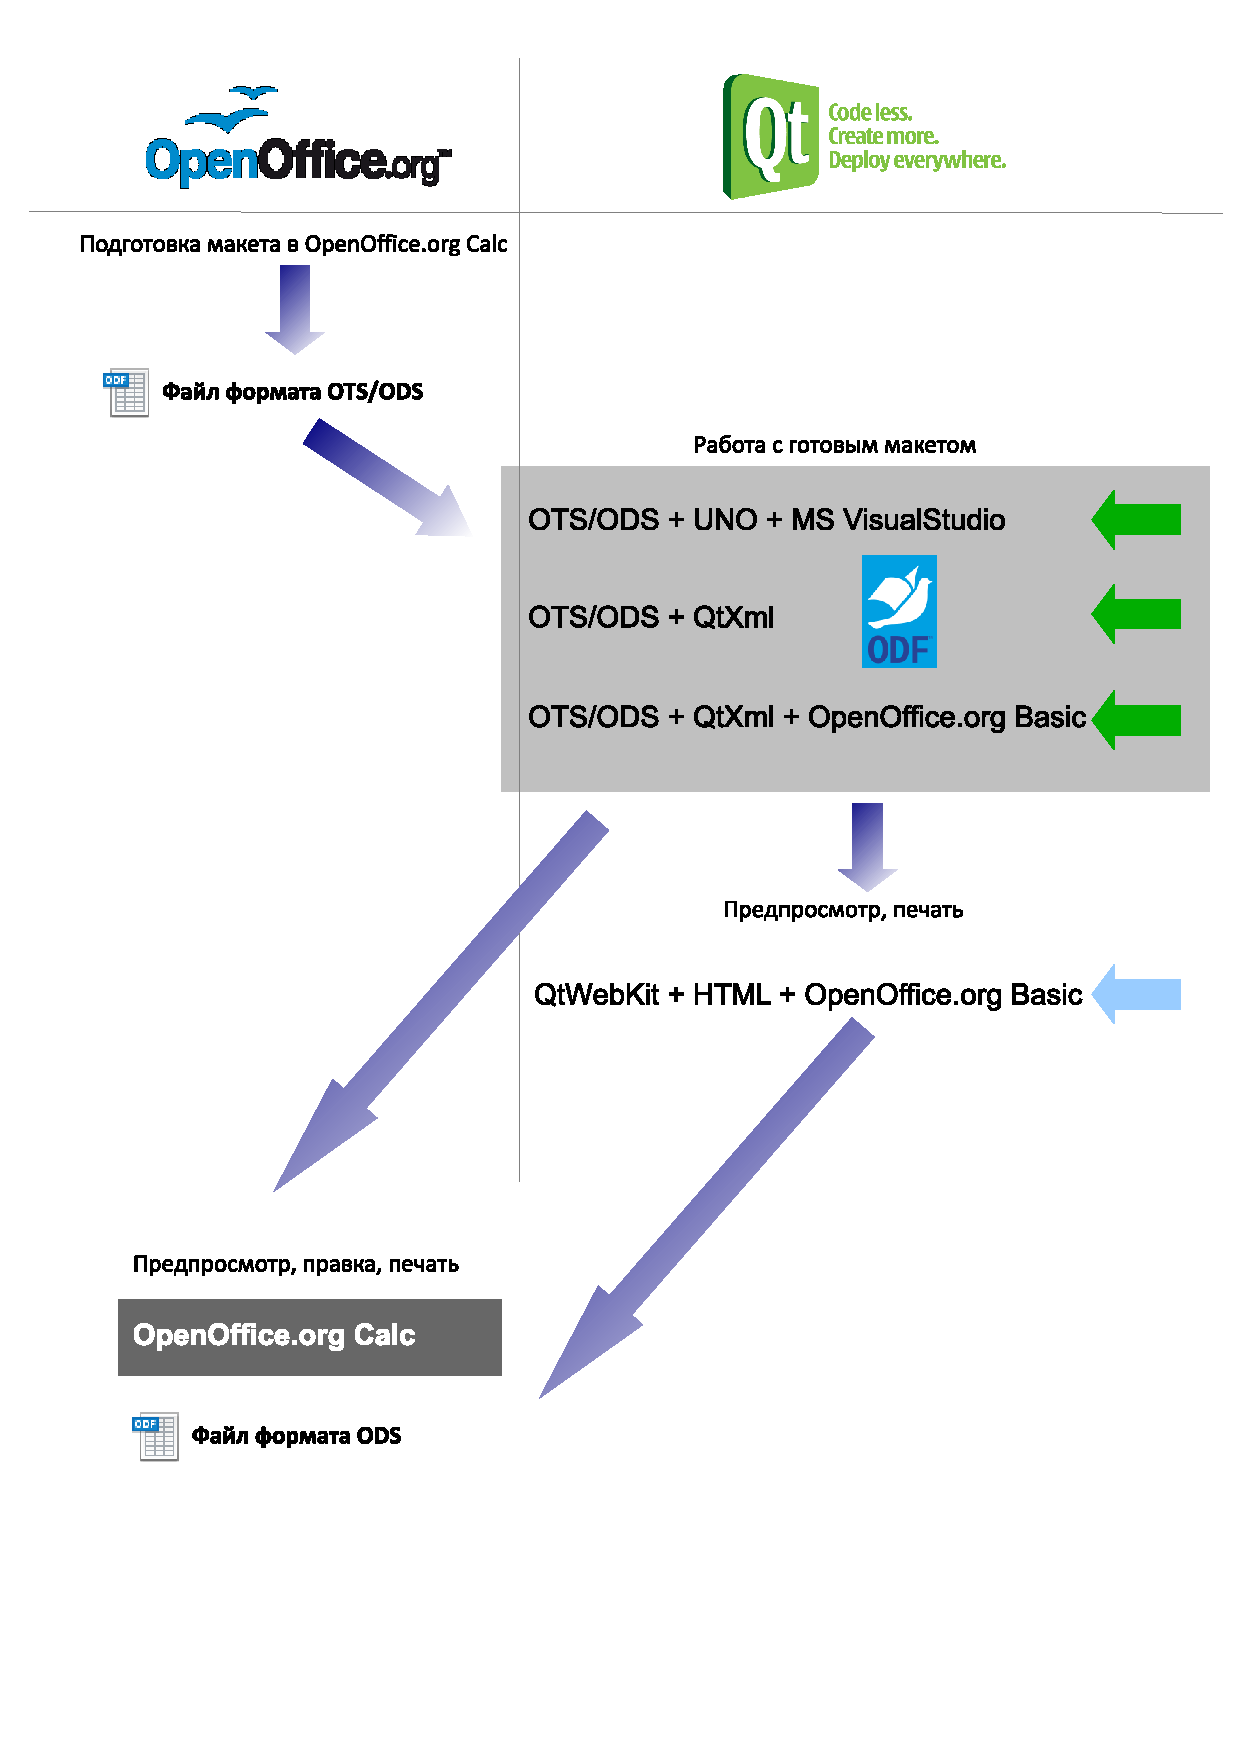
\includegraphics[height=0.6\textheight]{08_garanin}}
\end{figure}

\end{document}

\documentclass[10pt, a5paper]{article}
\usepackage{pdfpages}
\usepackage{parallel}
\usepackage[T2A]{fontenc}
\usepackage{ucs}
\usepackage[utf8x]{inputenc}
\usepackage[polish,english,russian]{babel}
\usepackage{hyperref}
\usepackage{rotating}
\usepackage[inner=2cm,top=1.8cm,outer=2cm,bottom=2.3cm,nohead]{geometry}
\usepackage{listings}
\usepackage{graphicx}
\usepackage{wrapfig}
\usepackage{longtable}
\usepackage{indentfirst}
\usepackage{array}
\newcolumntype{P}[1]{>{\raggedright\arraybackslash}p{#1}}
\frenchspacing
\usepackage{fixltx2e} %text sub- and superscripts
\usepackage{icomma} % коскі ў матэматычным рэжыме
\PreloadUnicodePage{4}

\newcommand{\longpage}{\enlargethispage{\baselineskip}}
\newcommand{\shortpage}{\enlargethispage{-\baselineskip}}

\def\switchlang#1{\expandafter\csname switchlang#1\endcsname}
\def\switchlangbe{
\let\saverefname=\refname%
\def\refname{Літаратура}%
\def\figurename{Іл.}%
}
\def\switchlangen{
\let\saverefname=\refname%
\def\refname{References}%
\def\figurename{Fig.}%
}
\def\switchlangru{
\let\saverefname=\refname%
\let\savefigurename=\figurename%
\def\refname{Литература}%
\def\figurename{Рис.}%
}

\hyphenation{admi-ni-stra-tive}
\hyphenation{ex-pe-ri-ence}
\hyphenation{fle-xi-bi-li-ty}
\hyphenation{Py-thon}
\hyphenation{ma-the-ma-ti-cal}
\hyphenation{re-ported}
\hyphenation{imp-le-menta-tions}
\hyphenation{pro-vides}
\hyphenation{en-gi-neering}
\hyphenation{com-pa-ti-bi-li-ty}
\hyphenation{im-pos-sible}
\hyphenation{desk-top}
\hyphenation{elec-tro-nic}
\hyphenation{com-pa-ny}
\hyphenation{de-ve-lop-ment}
\hyphenation{de-ve-loping}
\hyphenation{de-ve-lop}
\hyphenation{da-ta-ba-se}
\hyphenation{plat-forms}
\hyphenation{or-ga-ni-za-tion}
\hyphenation{pro-gramming}
\hyphenation{in-stru-ments}
\hyphenation{Li-nux}
\hyphenation{sour-ce}
\hyphenation{en-vi-ron-ment}
\hyphenation{Te-le-pathy}
\hyphenation{Li-nux-ov-ka}
\hyphenation{Open-BSD}
\hyphenation{Free-BSD}
\hyphenation{men-ti-on-ed}
\hyphenation{app-li-ca-tion}

\def\progref!#1!{\texttt{#1}}
\renewcommand{\arraystretch}{2} %Іначай формулы ў матрыцы зліпаюцца з лініямі
\usepackage{array}

\def\interview #1 (#2), #3, #4, #5\par{

\section[#1, #3, #4]{#1 -- #3, #4}
\def\qname{LVEE}
\def\aname{#1}
\def\q ##1\par{{\noindent \bf \qname: ##1 }\par}
\def\a{{\noindent \bf \aname: } \def\qname{L}\def\aname{#2}}
}

\def\interview* #1 (#2), #3, #4, #5\par{

\section*{#1\\{\small\rm #3, #4. #5}}

\def\qname{LVEE}
\def\aname{#1}
\def\q ##1\par{{\noindent \bf \qname: ##1 }\par}
\def\a{{\noindent \bf \aname: } \def\qname{L}\def\aname{#2}}
}


\begin{document}

\title{Базовая серверная архитектура для высоконагруженного стартапа}

\author{Михаил Пянко\\
\small Минск, ООО Анакреон,\texttt{mihail.pianko@warecorp.com}
}
\maketitle

\begin{abstract}
This article describes how to create a good environment for start-up project: what kind of server do we need for each role, and how these servers should communicate. Architecture restrictions are considered. Technical and architecture suggestions are made.
\end{abstract}

На начальном этапе разработки стартапа многие разработчики сталкиваются с проблемой создания достаточно гибкой и в будущем масштабируемой архитектуры приложения, оптимизированной для большой нагрузки. Мы хотели бы поделиться опытом в этой области. В качестве примера рассмотрим методы построения ресурса, базирующегося на Ruby On Rails. Тем не менее примеры, которые будут приведены ниже, с легкостью могут быть использованы для LAMP-решений. 

\section*{Серверы можно разделить на несколько типов по ролям:}
\begin{itemize}
\item Application
\item Database 
\item Load Balancer
\item Utils
\item Tools
\end{itemize}

{\bf Application} --- это frontend-сервер. Возможно использование как одного, так и нескольких Application-серверов. В случае использования одного Application-сервера надобности в балансировке нагрузки нет.

Application сервер выполняет следующие функции:
\begin{itemize}
\item обработка запросов от пользователей (получает запросы от балансировщика нагрузки),
\item взаимодействие с базой данных (Database server),
\item отправка сообщений в очередь сообщений (Utils server),
\item взаимодействие с CDN,
\item взаимодействие с search engines (Util server),
\item инвалидация кэша,
\item работа с кэшем (Database server).
\end{itemize}

Application сервер не должен производить следующих действий:
\begin{itemize}
\item преобразование медиа контента (видео, аудио, слайдшоу, и т.д.),
\item преобразование/кропинг картинок (если позволяет архитектура),
\item отправка сообщений электронной почты (если позволяет архитектура),
\item запросы на сторонние ресурсы через RestClient, curl, etc. (если позволяет архитектура).
\end{itemize}
{\bf Database} --- сервер, на котором находится база данных. В некоторых случаях на Database-сервер также устанавливается memcached, но это зависит от загрузки и конфигурации Database-сервера. 

Database-сервер выполняет следующие функции:
\begin{itemize}
\item обработка запросов от Application и Utils серверов,
\item хранение кэша (в случае установки memcached на DB сервер).
\end{itemize}
{\bf Load Balancer} --- балансировщик нагрузки, необходимый для распределения запросов пользователей между Application-серверами. Простейшим решением является использование nginx в качестве балансировщика нагрузки.

Load Balancer выполняет следующие функции:
\begin{itemize}
\item распределение запросов между Application серверами,
\item обработка HTTPS соединений (SSL сертификат должен быть сконфигурирован на балансировщике),
\item кэширование при использовании Varnish или связки nginx + memcache,
\item Firewall.
\end{itemize}

{\bf Utils} --- сервер, на котором располагаются сопутствующие сервисы, необходимые для отложенной обработки данных. Вот краткий список:
\begin{itemize}
\item message queue (RabbitMQ, Apache Message Queue, etc),
\item search engines (Solr, Sphinx, etc),
\item обработчики сообщений,
\item сервисы для обработки Video, Audio, SlideShow,
\item отправка сообщений электронной почты,
\item взаимодействие с CDN,
\item инвалидация кэша,
\item взаимодействие со сторонними ресурсами (PDF converters, \linebreak SendGrid, etc.). 
\end{itemize}
{\bf Tools} "--- сервер, необходимый для установки сторонних решений для работы приложения. В частности, приложения, базирующиеся на Java/Tomcat, система мониторинга и ресурсы, в безопасности которых вы сомневаетесь (Spellchecker, etc.). Tools-сервер не может установить соединения с Application, Database, Utils-серверами. Единственный протокол взаимодействия "--- это HTTP. Это дает гарантию того, что в результате взлома стороннего компонента основная ферма не пострадает. Сервер с этой ролью не обязателен. 


\begin{figure}[ht]
\centering{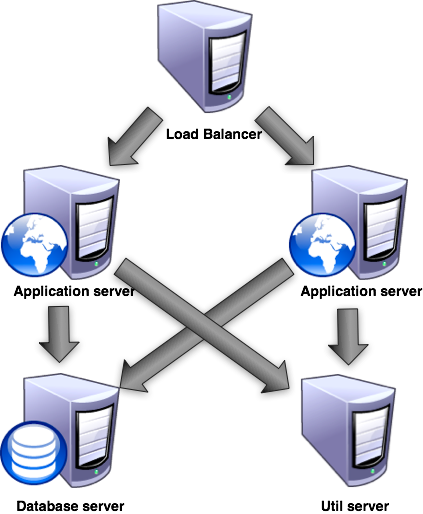
\includegraphics[width=8cm]{09_pianko.png}}
\label{pic:fl1}
%\caption{~}
\end{figure}

\section*{Ограничения, которые накладываются на архитектуру приложения}

\subsection*{Хранение кэша}
Необходимо организовать централизованное хранилище кэша. Файловый кэш и кэширование данных в памяти сервера работать не будет, так как кэш может создаваться и инвалидироваться с разных серверов. Наилучшим решением в данном случае является использования memcached. 

\subsection*{Хранение сессий пользователя}
В данном случае целесообразно хранить сессии в memcached или в Cookies. Отдача сессии на сторону пользователя --- менее безопасное и более медленное решение, чем хранение в memcached. 

\subsection*{Хранение медиа-данных пользователя}
Любой контент, загруженный пользователем на сервер, не может быть просто  сохранен в папку /public/upload. Наилучшим способом хранения данных является CDN. 

\subsection*{Рекомендации по автоматизированной конфигурации серверов}
Существует достаточно большое количество ПО для поддержания конфигурации серверов: Сfengine, Puppet, Chef, Sprinkle. 

Для автоматизированного конфигурирования серверов мы используем Sprinkle. Sprinkle --- это достаточно простое приложение на RoR, позволяющее разрабатывать сценарии по установке ПО на UNIX"=сервера.  Sprinkle поддерживает разделение серверов на роли, фермы и т.д. Так же поддерживаются различные типы инсталяторов, методов проверки текущей конфигурации, источников данных. Sprinkle имеет открытый исходный код, что позволяет вносить изменения в логику работы отдельных компонентов или создавать дополнительные модули. 

\section*{Варианты инсталляции}
Существует несколько вариантов ферм.
\begin{itemize}
\item Single server installation.
  \begin{itemize}
  \item На одном сервере располагаются Application + Util + Database
  \end{itemize}
\item Light farm
  \begin{itemize}
  \item $1$ сервер: Application 
  \item $1$ сервер: Util + DB
  \end{itemize}
\item Big farm:
  \begin{itemize}
  \item $1$ сервер: Load Ballancer 
  \item $x$ серверов: Application
  \item $1-x$ серверов: Util 
  \item $1-x$ серверов: Database (о репликациях и масштабировании базы данных можем поговорить чуть позже) 
  \end{itemize}
\end{itemize}
На самом деле существует множество комбинаций распределения ролей по физическим серверам. Необходимо выбирать оптимальный вариант в зависимости от нагрузки на сервера каждой роли. 

\section*{Рекомендации по архитектуре. Несколько примеров}

\subsection*{Интеграция со сторонними ресурсами}
Зачастую необходима интеграция со сторонними ресурсами для преобразования видео и аудио, обработки слайд-шоу, отсылки писем и т.д. 

Это подразумевает установку соединения по протоколам TCP, HTTP, etc. 
В данном случае существует несколько рисков:
\begin{itemize}
\item сервер недоступен
\item сервер перегружен 
\end{itemize}

В первом случае пользователь не сможет завершить действие, часть данных может быть потеряна или пользователь увидит сообщение ошибки на экране. 
Во втором случае мы получим очень долгую обработку страницы, что доставит неудобство пользователю. 

Лучшим решением в данном случае является отправка события в очередь сообщений и обработка на стороне util"=сервера. 

\subsection*{Обработка картинок пользователя}
Если ваш ресурс поддерживает возможность загрузки аватаров пользователей, логотипов с последующим ресайзингом изображений, вы можете столкнуться с проблемой большой нагрузки на сервер. 

Есть несколько распространенных методов ресайзинга изображений:

\begin{itemize}
\item оригинальное изображение сохраняется в хранилище без обработки. Доступ к изображению со страниц сайта реализован через врапер с элементарной логикой. Если картинка сгенерирована, то необходимо отдать ее через STDOUT или вернуть редирект на статический. Если картинка отсутствует, то сгенерировать и выполнить предыдущий шаг. Проблема этого метода в том, что нагрузка, которую может создать данный алгоритм, не может быть спрогнозирована.  При добавлении нового размера изображения достаточно визита поискового бота - и скорее всего сервера будут перегружены. 
\item оригинальное изображение преобразуется в нужные форматы и размеры непосредственно после загрузки на сервер. Это дает единовременную нагрузку на Application-сервера. Минусом данного метода является задержка в возврате страницы пользователю, что может вызвать дискомфорт.
\item последний вариант является модифицированной версией \linebreak предыдущего. Вместо непосредственной обработки изображения на Application-сервере необходимо отправить событие в очередь сообщения и произвести обработку изображения на Util"=сервере. 
\end{itemize}

\section*{Заключение}

Выше приведены приемы для построения начальной архитектуры высоконагруженной системы, которая в будущем может быть легко расширена и  смасштабирована. Способы дальнейшего развития напрямую зависят от архитектуры приложения, нагрузки на отдельные узлы системы и специфики проекта.

\end{document}





\documentclass[10pt, a5paper]{article}
\usepackage{pdfpages}
\usepackage{parallel}
\usepackage[T2A]{fontenc}
\usepackage{ucs}
\usepackage[utf8x]{inputenc}
\usepackage[polish,english,russian]{babel}
\usepackage{hyperref}
\usepackage{rotating}
\usepackage[inner=2cm,top=1.8cm,outer=2cm,bottom=2.3cm,nohead]{geometry}
\usepackage{listings}
\usepackage{graphicx}
\usepackage{wrapfig}
\usepackage{longtable}
\usepackage{indentfirst}
\usepackage{array}
\newcolumntype{P}[1]{>{\raggedright\arraybackslash}p{#1}}
\frenchspacing
\usepackage{fixltx2e} %text sub- and superscripts
\usepackage{icomma} % коскі ў матэматычным рэжыме
\PreloadUnicodePage{4}

\newcommand{\longpage}{\enlargethispage{\baselineskip}}
\newcommand{\shortpage}{\enlargethispage{-\baselineskip}}

\def\switchlang#1{\expandafter\csname switchlang#1\endcsname}
\def\switchlangbe{
\let\saverefname=\refname%
\def\refname{Літаратура}%
\def\figurename{Іл.}%
}
\def\switchlangen{
\let\saverefname=\refname%
\def\refname{References}%
\def\figurename{Fig.}%
}
\def\switchlangru{
\let\saverefname=\refname%
\let\savefigurename=\figurename%
\def\refname{Литература}%
\def\figurename{Рис.}%
}

\hyphenation{admi-ni-stra-tive}
\hyphenation{ex-pe-ri-ence}
\hyphenation{fle-xi-bi-li-ty}
\hyphenation{Py-thon}
\hyphenation{ma-the-ma-ti-cal}
\hyphenation{re-ported}
\hyphenation{imp-le-menta-tions}
\hyphenation{pro-vides}
\hyphenation{en-gi-neering}
\hyphenation{com-pa-ti-bi-li-ty}
\hyphenation{im-pos-sible}
\hyphenation{desk-top}
\hyphenation{elec-tro-nic}
\hyphenation{com-pa-ny}
\hyphenation{de-ve-lop-ment}
\hyphenation{de-ve-loping}
\hyphenation{de-ve-lop}
\hyphenation{da-ta-ba-se}
\hyphenation{plat-forms}
\hyphenation{or-ga-ni-za-tion}
\hyphenation{pro-gramming}
\hyphenation{in-stru-ments}
\hyphenation{Li-nux}
\hyphenation{sour-ce}
\hyphenation{en-vi-ron-ment}
\hyphenation{Te-le-pathy}
\hyphenation{Li-nux-ov-ka}
\hyphenation{Open-BSD}
\hyphenation{Free-BSD}
\hyphenation{men-ti-on-ed}
\hyphenation{app-li-ca-tion}

\def\progref!#1!{\texttt{#1}}
\renewcommand{\arraystretch}{2} %Іначай формулы ў матрыцы зліпаюцца з лініямі
\usepackage{array}

\def\interview #1 (#2), #3, #4, #5\par{

\section[#1, #3, #4]{#1 -- #3, #4}
\def\qname{LVEE}
\def\aname{#1}
\def\q ##1\par{{\noindent \bf \qname: ##1 }\par}
\def\a{{\noindent \bf \aname: } \def\qname{L}\def\aname{#2}}
}

\def\interview* #1 (#2), #3, #4, #5\par{

\section*{#1\\{\small\rm #3, #4. #5}}

\def\qname{LVEE}
\def\aname{#1}
\def\q ##1\par{{\noindent \bf \qname: ##1 }\par}
\def\a{{\noindent \bf \aname: } \def\qname{L}\def\aname{#2}}
}


\begin{document}
\title{Мониторинг Linux/FreeBSD серверов}
\author{Николай Маржан\footnote{Киев, Украина, PortaOne, Inc. \url{delgod@delgod.com}}}

\maketitle



\begin{abstract}Purposes and functions of monitoring systems are discussed, as far as general approaches to analyze the diagnostic parameters of a server. Observed information is classified into parameters received from hardware maintenance, operating system, services and typical database. Sample diagnostic parameters are presented for each category.
\end{abstract}

К стандартным целям проводимого на серверах мониторинга можно отнести:
\begin{itemize}
	\item Отслеживание критических значений диагностических параметров состояния и уведомление инженеров об их появлении.
	\item Накопление статистической информации для последующего анализа.
\end{itemize}

Уведомление о том, что система находится в критическом состоянии, является наиболее важной функцией мониторинга, так как требует немедленного вмешательства инженеров, которые занимаются поддержкой данной системы.

Даже если проблема носит временный характер (например, стопроцентная загрузка процессора, возникшая спонтанно и затем прекратившаяся через 20 минут), выяснить причину такого поведения можно только тогда, когда проблема присутствует (причиной могла быть удаленная DOS-атака).

Накопление статистической информации происходит обычно в 2-х видах:
\begin{itemize}
	\item Лог-файлы. Обычно в них записываются только те моменты, когда система входит в критическое состояние, и когда возващается в нормальное.
	\item Данные для графиков по каждому показателю.
\end{itemize}

Графики --- не менее важная часть системы мониторинга, так как только они позволяют проводить анализ состояния сервера в целом, как сложной системы. 
Используя графики для наблюдения динамики диагностических параметров, мы можем:
\begin{itemize}
	\item Увидеть, в каком состоянии находился сервер в любой момент времени в прошлом. Мы можем быстро понять, чем отличается сегодняшнее состояние от состояния недельной давности.
	\item Проследить закономерности возможной взаимосвязи между диагностическими параметрами. Например, когда повышается входящий трафик на сетевом интерфейсе --- повышается нагрузка на центральный процессор.
	\item Находить противоречия между значениями диагностических параметров. Например, сильно возросло количество запросов на чтение к базе данных, и база данных начала использовать на 1 Гб больше оперативной памяти, но при этом с жесткого диска было считано всего 100 Мб данных.
 Увидеть, в каком состоянии находился сервер в любой момент времени в прошлом. Мы можем быстро понять, чем отличается сегодняшнее состояние от состояния недельной давности.
	\item Проследить закономерности возможной взаимосвязи между диагностическими параметрами. Например, когда повышается входящий трафик на сетевом интерфейсе --- повышается нагрузка на центральный процессор.
	\item Находить противоречия между значениями диагностических параметров. Например, сильно возросло количество запросов на чтение к базе данных, и база данных начала использовать на 1 Гб больше оперативной памяти, но при этом с жесткого диска было считано всего 100 Мб данных.
\end{itemize}
Диагностическими параметрами состояния для аппаратного обеспечения являются: 
\begin{enumerate}
	\item температура центрального процессора;
	\item наличие повреждённых секторов или ошибок чтения на жестком диске;
	\item состояние аппаратного RAID-контроллера.
\end{enumerate}
К диагностическим параметрам состояния для операционной системы можно отнести:
\begin{enumerate}
	\item количество задач, ожидающих выполнения (load average);
	\item время простоя центрального процессора (idle);
	\item время простоя каждого ядра центрального процессора (idle);
	\item размер свободного места на жестком диске;
	\item нагрузка на жесткий диск;
	\item количество данных в разделе подкачки (swap);
	\item активная запись или чтение с раздела подкачки (swaping/paging);
	\item количество использованной памяти;
	\item количество памяти, потребляемой каждым приложением;
	\item скорость передачи данных на сетевых интерфейсах;
	\item подтверждение того, что сетевые интерфейсы работают на нужной скорости и в полнодуплексном режиме;
	\item количество ошибок и коллизий на сетевых интерфейсах;
	\item состояние системных буферов (freebsd vm.zone), mbuf clusters, sendfile-буферов, размер KVM, Pipe KVA;
	\item количество открытых файлов, количество открытых сокетов;
	\item отсутствие процессов-зомби;
	\item отсутствие ошибок сегментации у процессов.
\end{enumerate}
Диагностическими параметрами состояния сервисов являются:
\begin{enumerate}
	\item подтверждение того, что все критически важные сервисы запущены.
	\item подтверждение того, что сервисы успевают вычитывать данные из входящей очереди сетевой подсистемы.
	\item подтверждение того, что нет отброшенных данных вследствие полных буферов соединения (dropped due to full socket buffers).
\end{enumerate}
Диагностическими параметрами состояния базы данных MySQL являются:
\begin{enumerate}
	\item количество максимально использованных соединений;
	\item количество запросов, количество медленных запросов;
	\item количество операций записи/чтения с жесткого диска;
	\item отставание репликации.
\end{enumerate}
Как показал опыт построения систем мониторинга в гетерогенных сетях, подходы и диагностические параметры практически идентичны для операционных систем FreeBSD и Linux; основные различия связаны с мониторингом системных буферов и с некоторыми расхождениями в синтаксисе команд.
\end{document}


\newpage

\makeatletter
\let\enddocument\@lvee@enddoc
\let\input\@lvee@input
\makeatother

\eof


